\documentclass[12pt]{article}

\usepackage{amsmath}
\usepackage{amssymb}
\usepackage[dvips]{graphicx}
\usepackage{eepic}
\usepackage{color}
\usepackage{wasysym} % \female \male
\usepackage[landscape,pdftex]{geometry}
\usepackage{fancyhdr}
\usepackage{hyperref}

\definecolor{cantelope}{rgb}{1.0,0.8,0.4}
\hypersetup{
    colorlinks, urlcolor={cantelope}
}
\hypersetup{pdfpagemode=UseNone} % don't show bookmarks on initial view

\DeclareOption{bigsym}{\DeclareSymbolFont{largesymbols}{OMX}{psycm}{m}{n}}
\ProcessOptions

\setlength{\oddsidemargin}{-0.75in}
\setlength{\evensidemargin}{-0.75in}
\setlength{\topmargin}{-1in}
\setlength{\textheight}{7.75in}
\setlength{\textwidth}{10.5in}
\setlength{\footskip}{0in}
\setlength{\parindent}{0pt}
\setlength{\rightskip}{0pt plus 1fil} % makes ragged right

\renewcommand{\familydefault}{phv} % helvetica

% following: color
\definecolor{mybgcolor}{rgb}{0,0,0.3125}
\definecolor{myyellow}{rgb}{1,1,0.4}
\definecolor{myblue}{rgb}{0.4,0.8,1}
\definecolor{mypink}{rgb}{1,0.4,1}
\definecolor{mywhite}{rgb}{1,1,1}

% header/footer layout
\pagestyle{fancy}
\lhead{} \chead{} \rhead{}
\lfoot{} \cfoot{} \rfoot{\color{myyellow} \thepage}
\renewcommand{\headrulewidth}{0pt}
\renewcommand{\footrulewidth}{0pt}

% font sizes
\newcommand{\superlarge}{\fontsize{60}{60} \selectfont}
\newcommand{\titlesize}{\fontsize{40}{50} \selectfont}
\newcommand{\headsize}{\fontsize{35}{35} \selectfont}
\newcommand{\textsize}{\fontsize{30}{35} \selectfont}
\newcommand{\smallsize}{\fontsize{25}{30} \selectfont}
\newcommand{\smallersize}{\fontsize{20}{25} \selectfont}
\newcommand{\smallestsize}{\fontsize{18}{22} \selectfont}
\newcommand{\lod}{\text{LOD}}
\newcommand{\plod}{\text{pLOD}}
\newcommand{\bic}{\text{BIC}}
\newcommand{\rss}{\text{RSS}}
\newcommand{\var}{\text{var}}
\newcommand{\M}{\text{M}}


\pagecolor{mybgcolor}
\color{mywhite}

\begin{document}
\thispagestyle{empty}

\begin{center}
\titlesize \color{myyellow}


\vspace*{15mm}

R/qtl Workshop

\color{mypink}
\rule{10in}{1mm}

\vspace{5mm}

\textsize \color{myblue}
Karl Broman
\vspace{5mm}

\color{mywhite}
{\smallsize Biostatistics and Medical Informatics

University of Wisconsin -- Madison
\vspace{20mm}


\href{http://rqtl.org}{\tt rqtl.org} \\[3pt]
\href{http://kbroman.org}{\tt kbroman.org} \\[3pt]
\href{https://github.com/kbroman}{\tt github.com/kbroman} \\
\href{https://twitter.com/kwbroman}{\tt @kwbroman}
}

\end{center}

\newpage

\headsize \color{myyellow}
\hfill \begin{minipage}{5.75in}
\centering
Backcross
\end{minipage}

\vfill

\centerline{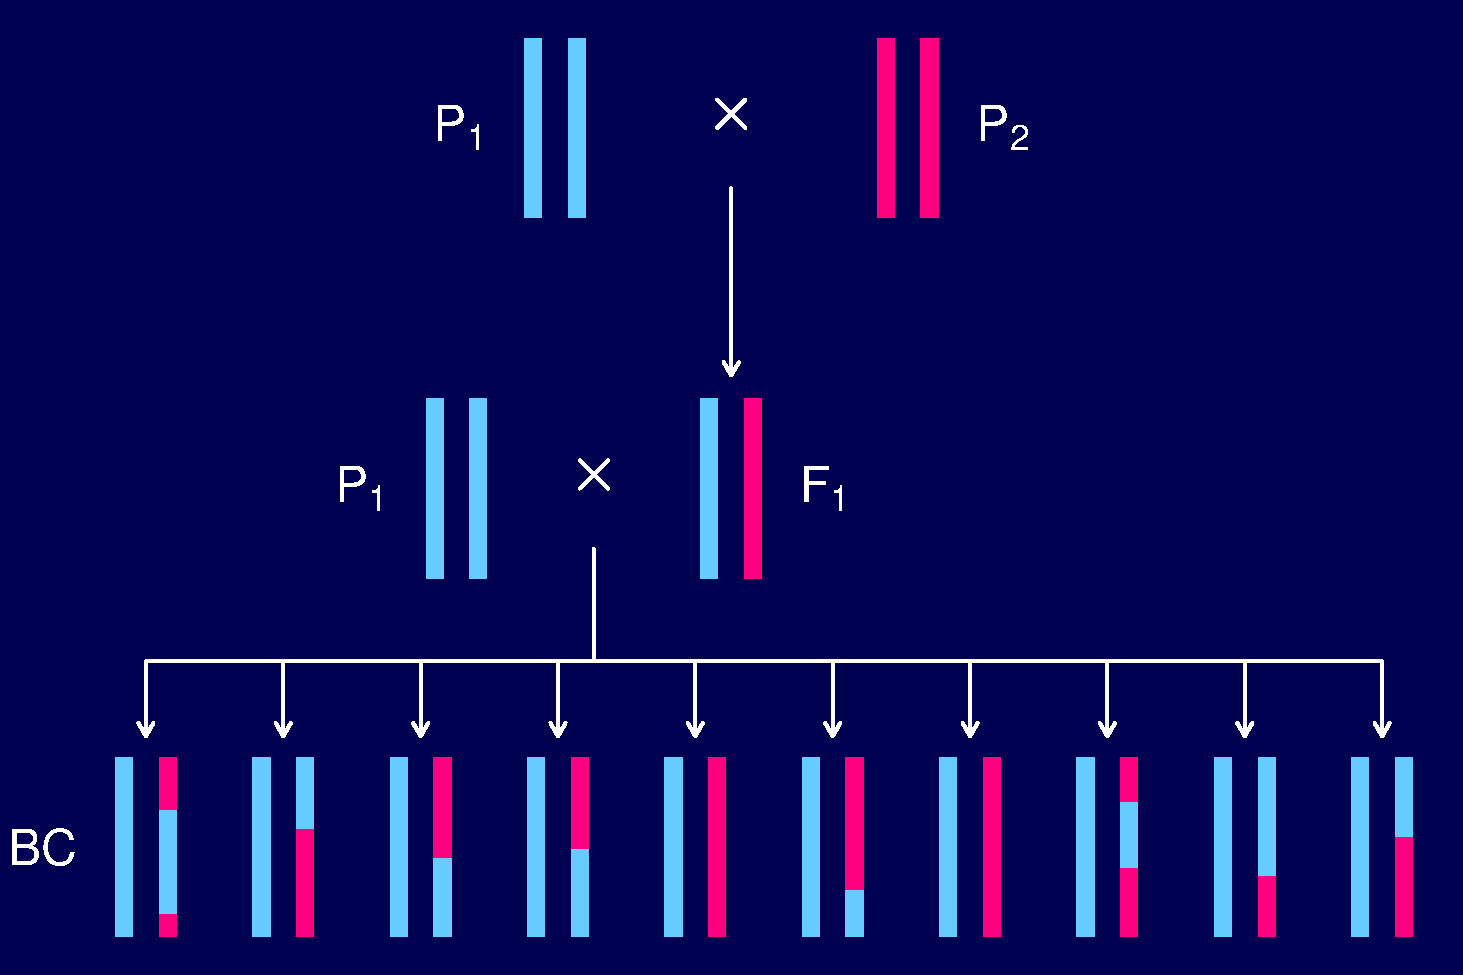
\includegraphics{FigsA/backcross.pdf}}

\newpage

\headsize \color{myyellow}
\hfill \begin{minipage}{5.75in}
\centering
Intercross
\end{minipage}

\vfill

\centerline{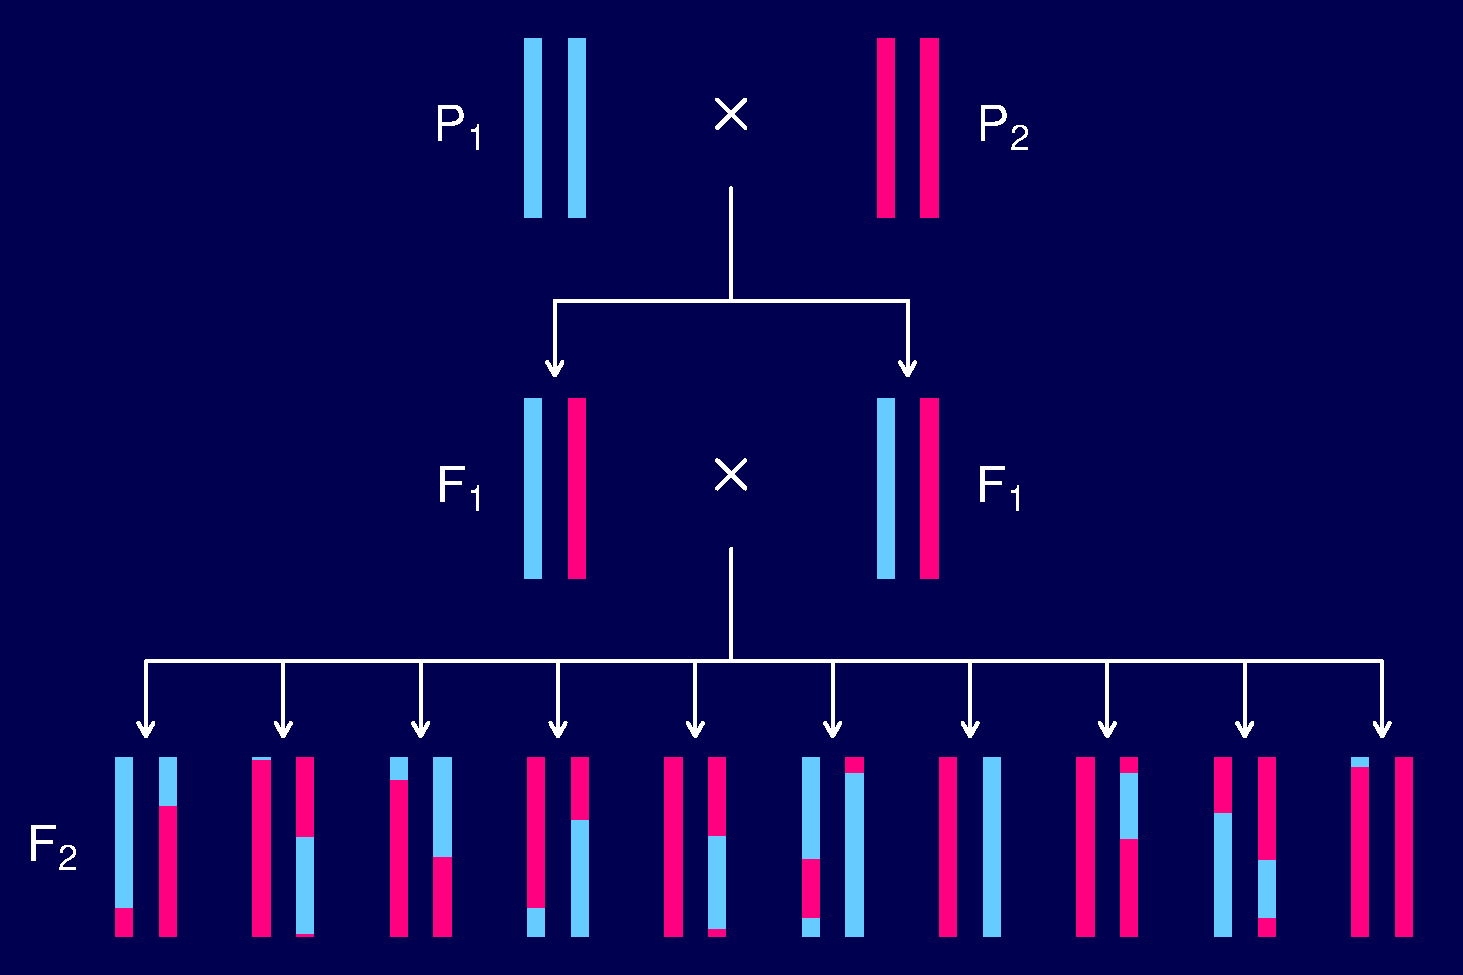
\includegraphics{FigsA/intercross.pdf}}

\newpage

\headsize \color{myyellow}
\hfill \begin{minipage}{5.75in}
\centering
Goals
\end{minipage}

\vspace{3cm}

\color{mywhite} \smallsize

\hfill \begin{minipage}[t]{9.5in}
\begin{itemize}
\itemsep24pt
\item Identify quantitative trait loci (QTL)\\[6pt]
   {\color{myblue}   (and interactions among QTL)}
\item Interval estimates of QTL location
\item Estimated QTL effects
\end{itemize} \end{minipage}


\newpage

\headsize \color{myyellow}
$\boldsymbol{\rightarrow}$ R

\vspace{3cm}

\color{mywhite} \smallsize

\hfill \begin{minipage}[t]{9.5in}
\begin{itemize}
\itemsep24pt
\item R, RStudio, and R/qtl
\item \verb|read.cross()|
\item \verb|summary()|, \verb|plot()|
\item \verb|nind()|, \verb|nmar()|, \verb|totmar()|, \verb|nchr()|
\end{itemize} \end{minipage}





\newpage

\headsize \color{myyellow}
\hfill\begin{minipage}{5.75in}
\centering
ANOVA at marker loci
\end{minipage}

\vspace{2cm}

\color{mywhite} \smallsize

\hspace*{0.5in}
\begin{minipage}[t]{4.1in}
\vspace*{5mm}

\sloppy
\smallersize
\begin{itemize}
\setlength{\rightskip}{0pt plus 1fil} % makes ragged right
\item Also known as {\color{mypink} marker regression}.
\item Split mice into groups according to genotype at a marker.
\item Do a t-test / ANOVA.
\item Repeat for each marker.
\end{itemize}
\end{minipage}
\hfill
\begin{minipage}[t]{5.3in}
\vspace*{0mm}

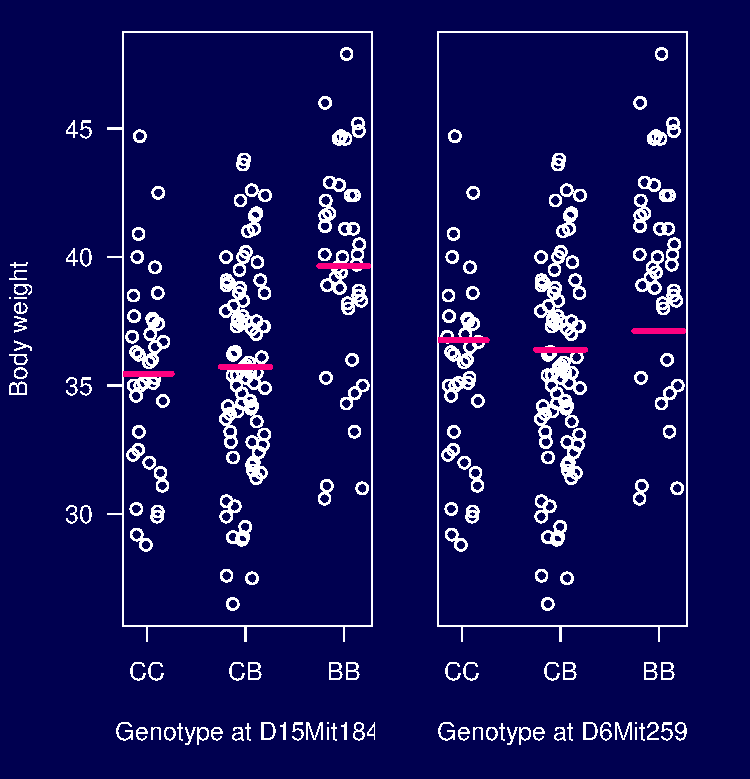
\includegraphics{FigsA/anova.pdf}
\end{minipage}







\newpage

\headsize \color{myyellow}
\hfill \begin{minipage}{5.75in}
\centering
ANOVA at marker loci
\end{minipage}

\vspace{2cm}

\color{mywhite} \smallsize

\hspace*{0.5in}
\begin{minipage}[t]{4.8in}
\textsize {\color{mypink} Advantages}

\smallersize \color{mywhite}
\begin{itemize}
\setlength{\rightskip}{0pt plus 1fil} % makes ragged right
\item Simple.
\item Easily incorporates covariates.
\item Easily extended to more complex models.
\item Doesn't require a genetic map.
\end{itemize}
\end{minipage}
\hfill
\begin{minipage}[t]{4.8in}
\textsize {\color{mypink} Disadvantages}

\smallersize \color{mywhite}
\begin{itemize}
\setlength{\rightskip}{0pt plus 1fil} % makes ragged right
\item Must exclude individuals with missing genotype data.
\item Imperfect information about QTL location.
\item Suffers in low density scans.
\item {\color{mypink} Only considers one QTL at a time.}
\end{itemize}
\end{minipage}






\newpage

\headsize \color{myyellow}
\hfill \begin{minipage}{5.75in}
\centering
Interval mapping
\end{minipage}

\vspace{15mm}

\hspace*{0.5in}
\color{mywhite} \smallsize
Lander \& Botstein (1989)
\vspace{1cm}

\smallersize
\hfill \begin{minipage}{9.5in}
\begin{itemize}
\itemsep24pt
\setlength{\rightskip}{0pt plus 1fil} % makes ragged right
  \item Assume a {\color{mypink} single} QTL model.
  \item Each position in the genome, one at a time, is posited as the
  putative QTL.
  \item Let $\mathsf{q = }$ the unobserved QTL genotype \\
        Assume $\mathsf{y | q \sim N(\mu_q, \sigma)}$
  \item We don't know $\mathsf{q}$, but we can calculate
    $\mathsf{\Pr(q \ | \ \text{marker data})}$
  \item Estimate $\mathsf{\mu_q, \sigma}$ by \emph{maximum likelihood}
    using an iterative EM algorithm
\end{itemize}
\end{minipage}



\newpage

\headsize \color{myyellow}
\hfill \begin{minipage}{5.75in}
\centering
Genotype probabilities
\end{minipage}

\vspace{15mm}

\centerline{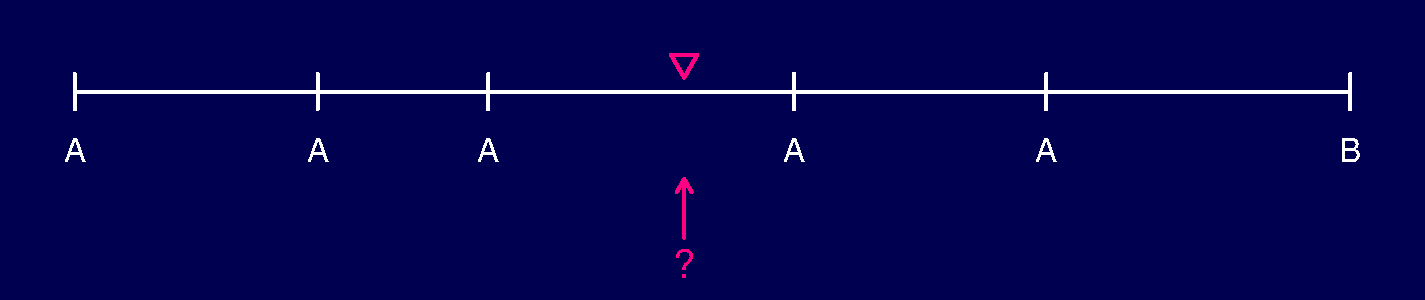
\includegraphics{FigsA/genoprob1.pdf}}

\vspace{15mm}

\hfill
\begin{minipage}{10in}
\color{mywhite} \smallersize
Calculate {\color{myblue} $\mathsf{\Pr(q \ | \ \text{marker data})}$}, assuming
\begin{itemize}
\item No crossover interference
\item No genotyping errors
\end{itemize}

\vspace{10mm}

Or use the {\color{mypink} hidden Markov model (HMM)} technology
\begin{itemize}
\item To allow for genotyping errors
\item To incorporate dominant markers
\item {\color{myblue} (Still assume no crossover interference.)}
\end{itemize}
\end{minipage}



\newpage

\addtocounter{page}{-1}

\headsize \color{myyellow}
\hfill \begin{minipage}{5.75in}
\centering
Genotype probabilities
\end{minipage}

\vspace{15mm}

\centerline{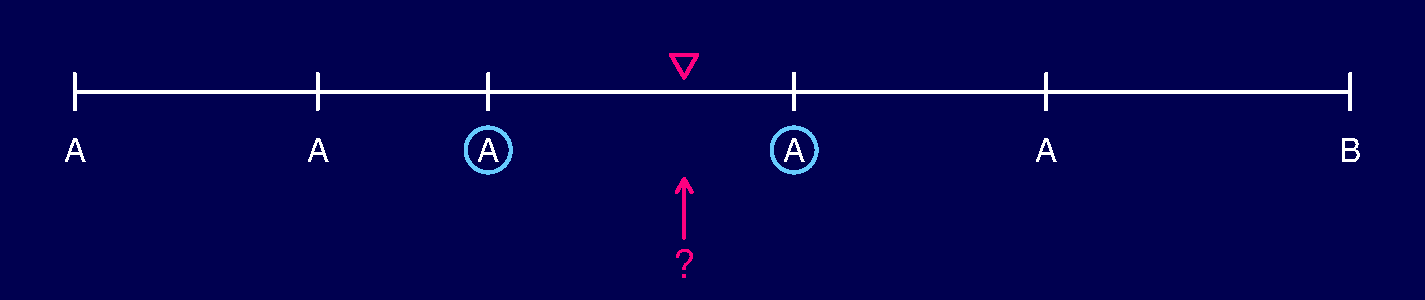
\includegraphics{FigsA/genoprob2.pdf}}

\vspace{15mm}

\hfill
\begin{minipage}{10in}
\color{mywhite} \smallersize
Calculate {\color{myblue} $\mathsf{\Pr(q \ | \ \text{marker data})}$}, assuming
\begin{itemize}
\item No crossover interference
\item No genotyping errors
\end{itemize}

\vspace{10mm}

Or use the {\color{mypink} hidden Markov model (HMM)} technology
\begin{itemize}
\item To allow for genotyping errors
\item To incorporate dominant markers
\item {\color{myblue} (Still assume no crossover interference.)}
\end{itemize}
\end{minipage}

\newpage

\addtocounter{page}{-1}

\headsize \color{myyellow}
\hfill \begin{minipage}{5.75in}
\centering
Genotype probabilities
\end{minipage}

\vspace{15mm}

\centerline{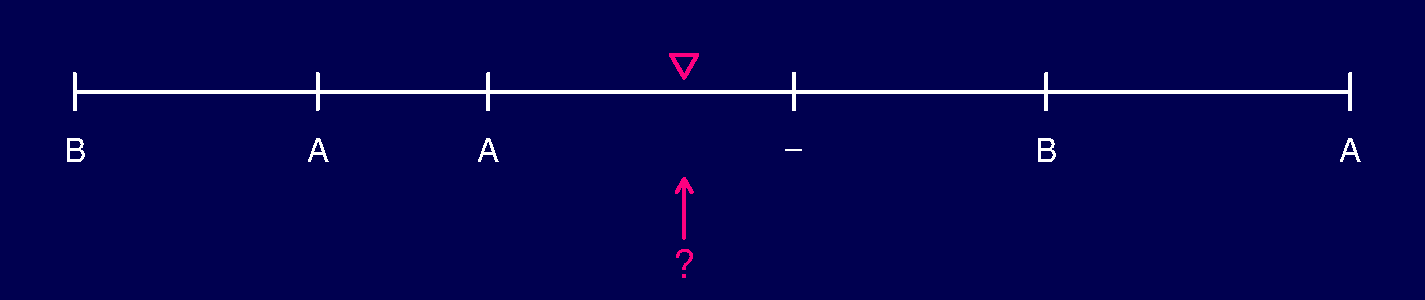
\includegraphics{FigsA/genoprob3.pdf}}

\vspace{15mm}

\hfill
\begin{minipage}{10in}
\color{mywhite} \smallersize
Calculate {\color{myblue} $\mathsf{\Pr(q \ | \ \text{marker data})}$}, assuming
\begin{itemize}
\item No crossover interference
\item No genotyping errors
\end{itemize}

\vspace{10mm}

Or use the {\color{mypink} hidden Markov model (HMM)} technology
\begin{itemize}
\item To allow for genotyping errors
\item To incorporate dominant markers
\item {\color{myblue} (Still assume no crossover interference.)}
\end{itemize}
\end{minipage}


\newpage

\addtocounter{page}{-1}

\headsize \color{myyellow}
\hfill \begin{minipage}{5.75in}
\centering
Genotype probabilities
\end{minipage}

\vspace{15mm}

\centerline{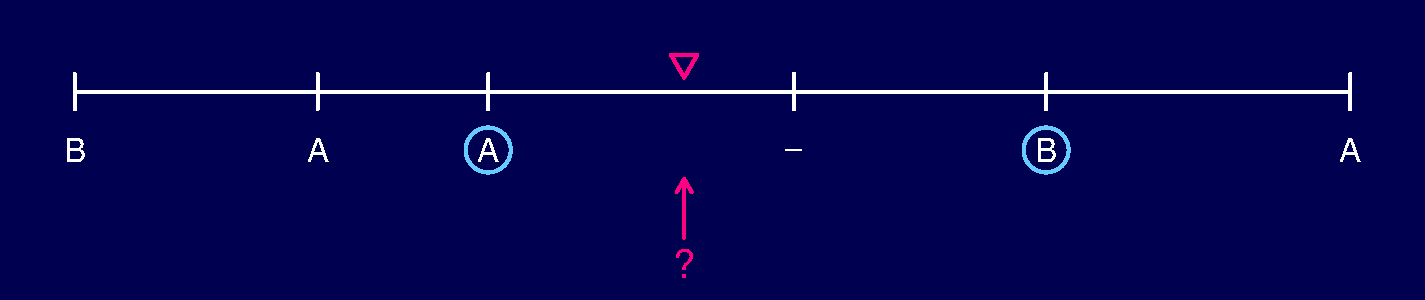
\includegraphics{FigsA/genoprob4.pdf}}

\vspace{15mm}

\hfill
\begin{minipage}{10in}
\color{mywhite} \smallersize
Calculate {\color{myblue} $\mathsf{\Pr(q \ | \ \text{marker data})}$}, assuming
\begin{itemize}
\item No crossover interference
\item No genotyping errors
\end{itemize}

\vspace{10mm}

Or use the {\color{mypink} hidden Markov model (HMM)} technology
\begin{itemize}
\item To allow for genotyping errors
\item To incorporate dominant markers
\item {\color{myblue} (Still assume no crossover interference.)}
\end{itemize}
\end{minipage}


\newpage

\addtocounter{page}{-1}

\headsize \color{myyellow}
\hfill \begin{minipage}{5.75in}
\centering
Genotype probabilities
\end{minipage}

\vspace{15mm}

\centerline{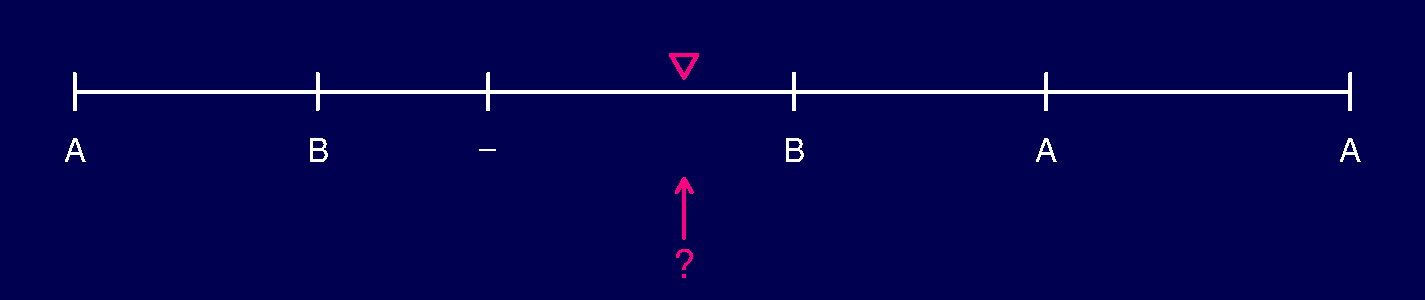
\includegraphics{FigsA/genoprob5.pdf}}

\vspace{15mm}

\hfill
\begin{minipage}{10in}
\color{mywhite} \smallersize
Calculate {\color{myblue} $\mathsf{\Pr(q \ | \ \text{marker data})}$}, assuming
\begin{itemize}
\item No crossover interference
\item No genotyping errors
\end{itemize}

\vspace{10mm}

Or use the {\color{mypink} hidden Markov model (HMM)} technology
\begin{itemize}
\item To allow for genotyping errors
\item To incorporate dominant markers
\item {\color{myblue} (Still assume no crossover interference.)}
\end{itemize}
\end{minipage}


\newpage

\addtocounter{page}{-1}

\headsize \color{myyellow}
\hfill \begin{minipage}{5.75in}
\centering
Genotype probabilities
\end{minipage}

\vspace{15mm}

\centerline{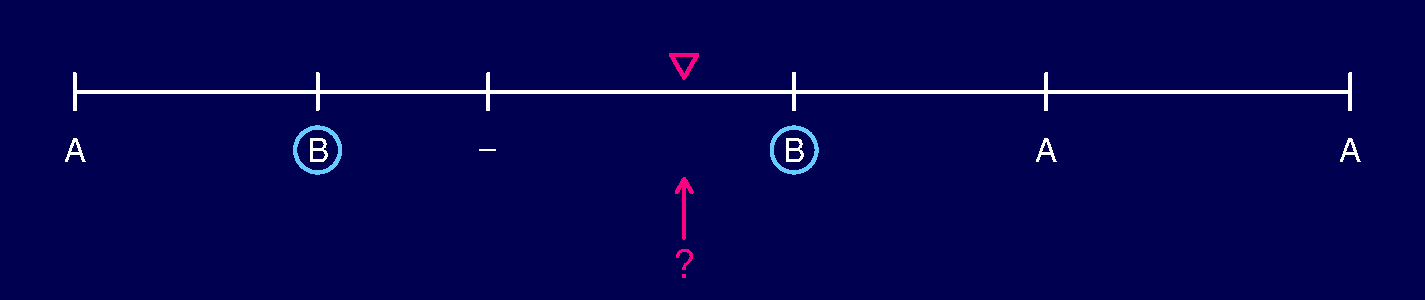
\includegraphics{FigsA/genoprob6.pdf}}

\vspace{15mm}

\hfill
\begin{minipage}{10in}
\color{mywhite} \smallersize
Calculate {\color{myblue} $\mathsf{\Pr(q \ | \ \text{marker data})}$}, assuming
\begin{itemize}
\item No crossover interference
\item No genotyping errors
\end{itemize}

\vspace{10mm}

Or use the {\color{mypink} hidden Markov model (HMM)} technology
\begin{itemize}
\item To allow for genotyping errors
\item To incorporate dominant markers
\item {\color{myblue} (Still assume no crossover interference.)}
\end{itemize}
\end{minipage}





\newpage

\headsize \color{myyellow}
\hfill \begin{minipage}{5.75in}
\centering
LOD scores
\end{minipage}

\vspace{25mm}

\hfill
\begin{minipage}{10in}
\color{mywhite} \smallersize
 The LOD score is a measure of the {\color{mypink} strength of
evidence} for the presence of a QTL at a particular
location.
\vspace{15mm}

 $\mathsf{\lod(\lambda)}$
\begin{minipage}[t]{8.5in}
$\mathsf{= \log_{10}}$ likelihood ratio comparing the hypothesis of a \\
\hspace*{8mm} QTL at position $\mathsf{\lambda}$ versus that of no QTL
\vspace{5mm}

\headsize
$\mathsf{= \log_{10} \left\{ \frac{\Pr(y | \text{QTL at $\lambda$}, \hat{\mu}_{0\lambda},
\hat{\mu}_{1\lambda}, \hat{\sigma}_\lambda)}{\Pr(y | \text{no QTL}, \hat{\mu},
\hat{\sigma})} \right\}}$
\end{minipage}
\vspace{15mm}

 $\mathsf{\hat{\mu}_{0\lambda}, \hat{\mu}_{1\lambda}, \hat{\sigma}_\lambda}$ are the MLEs,
assuming a single QTL at position $\mathsf{\lambda}$.
\vspace{15mm}

 No QTL model:
\begin{minipage}[t]{7.5in}
The phenotypes are independent and identically
distributed (iid) $\mathsf{N(\mu, \sigma^2)}$.
\end{minipage}
\end{minipage}





\newpage

\headsize \color{myyellow}
$\boldsymbol{\rightarrow}$ R

\vspace{3cm}

\color{mywhite} \smallsize

\hfill \begin{minipage}[t]{9.5in}
\begin{itemize}
\itemsep24pt
\item \verb|calc.genoprob()|
\item \verb|scanone()|
\item \verb|iplotScanone()| from \href{http://kbroman.org/qtlcharts}{R/qtlcharts}
\end{itemize} \end{minipage}





\newpage

\headsize \color{myyellow}
\hfill \begin{minipage}{5.75in}
\centering
Interval mapping
\end{minipage}

\vspace{2cm}

\color{mywhite} \smallsize

\hspace*{0.5in}
\begin{minipage}[t]{4.8in}
\textsize {\color{mypink} Advantages}

\smallersize \color{mywhite}
\begin{itemize}
\setlength{\rightskip}{0pt plus 1fil} % makes ragged right
\item Takes proper account of missing data.
\item Allows examination of positions between markers.
\item Gives improved estimates of QTL effects.
\item Provides pretty graphs.
\end{itemize}
\end{minipage}
\hfill
\begin{minipage}[t]{4.8in}
\textsize {\color{mypink} Disadvantages}

\smallersize \color{mywhite}
\begin{itemize}
\setlength{\rightskip}{0pt plus 1fil} % makes ragged right
\item Increased computation time.
\item Requires specialized software.
\item Difficult to generalize.
\item {\color{mypink} Only considers one QTL at a time.}
\end{itemize}
\end{minipage}




\newpage

\headsize \color{myyellow}
\hfill \begin{minipage}{5.75in}
\centering
LOD thresholds
\end{minipage}

\smallersize \color{mywhite}

\vspace{25mm}

\hfill
\begin{minipage}{10in}
Large LOD scores indicate evidence for the presence of a QTL
\vspace{5mm}

{\color{mypink} Question}: How large is large?
\vspace{20mm}

{\color{myyellow} LOD threshold} =  \hspace{2mm}
\begin{minipage}[t]{7in}
\setlength{\rightskip}{0pt plus 1fil} % makes ragged right
95 \%ile of distr'n of max LOD, genome-wide, if there are no QTLs anywhere
\end{minipage}
\vspace{20mm}

\hspace{15mm} {\color{myyellow} Derivation:} \hfill
\begin{minipage}[t]{7.5in}
\begin{itemize}
\item Analytical calculations (L \& B 1989)
\item Simulations (L \& B 1989)
\item Permutation tests (Churchill \& Doerge 1994)
\end{itemize} \end{minipage}
\end{minipage}



\newpage

\headsize \color{myyellow}
\hfill \begin{minipage}{5.75in}
\centering
Null distribution of the LOD score
\end{minipage}

\vspace{3cm}

\hspace*{0.5in}
\begin{minipage}[t]{4.7in}
\vspace*{10mm}

\color{mywhite} \smallersize
\begin{itemize}
\setlength{\rightskip}{0pt plus 1fil} % makes ragged right
\item Null distribution derived by computer simulation of backcross
with genome of typical size.
\item Dashed curve: distribution of LOD score at any one point.
\item Solid curve: distribution of maximum LOD score, genome-wide.
\end{itemize}
\end{minipage}
\hfill
\begin{minipage}[t]{4.7in}
\vspace*{0cm}

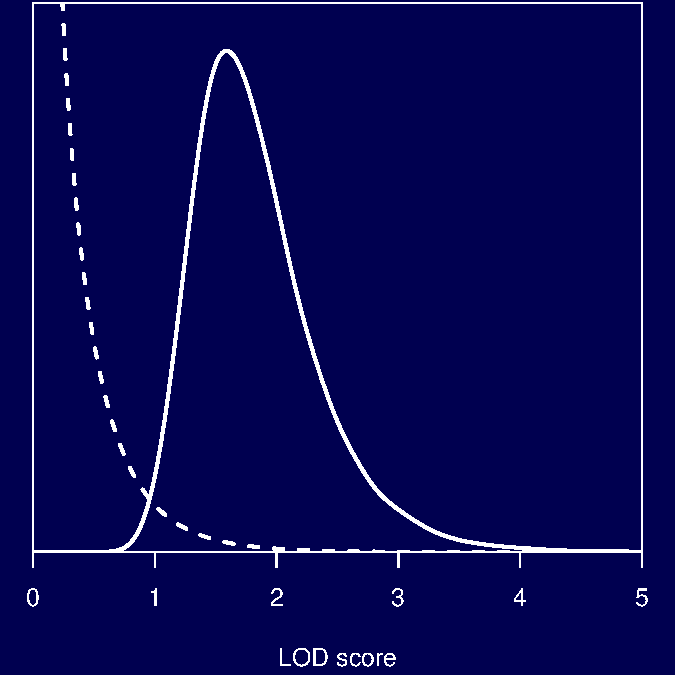
\includegraphics{FigsA/loddist.pdf}
\end{minipage}








\newpage

\headsize \color{myyellow}
\hfill \begin{minipage}{5.75in}
\centering
Permutation test
\end{minipage}

\vspace{2cm}

\centerline{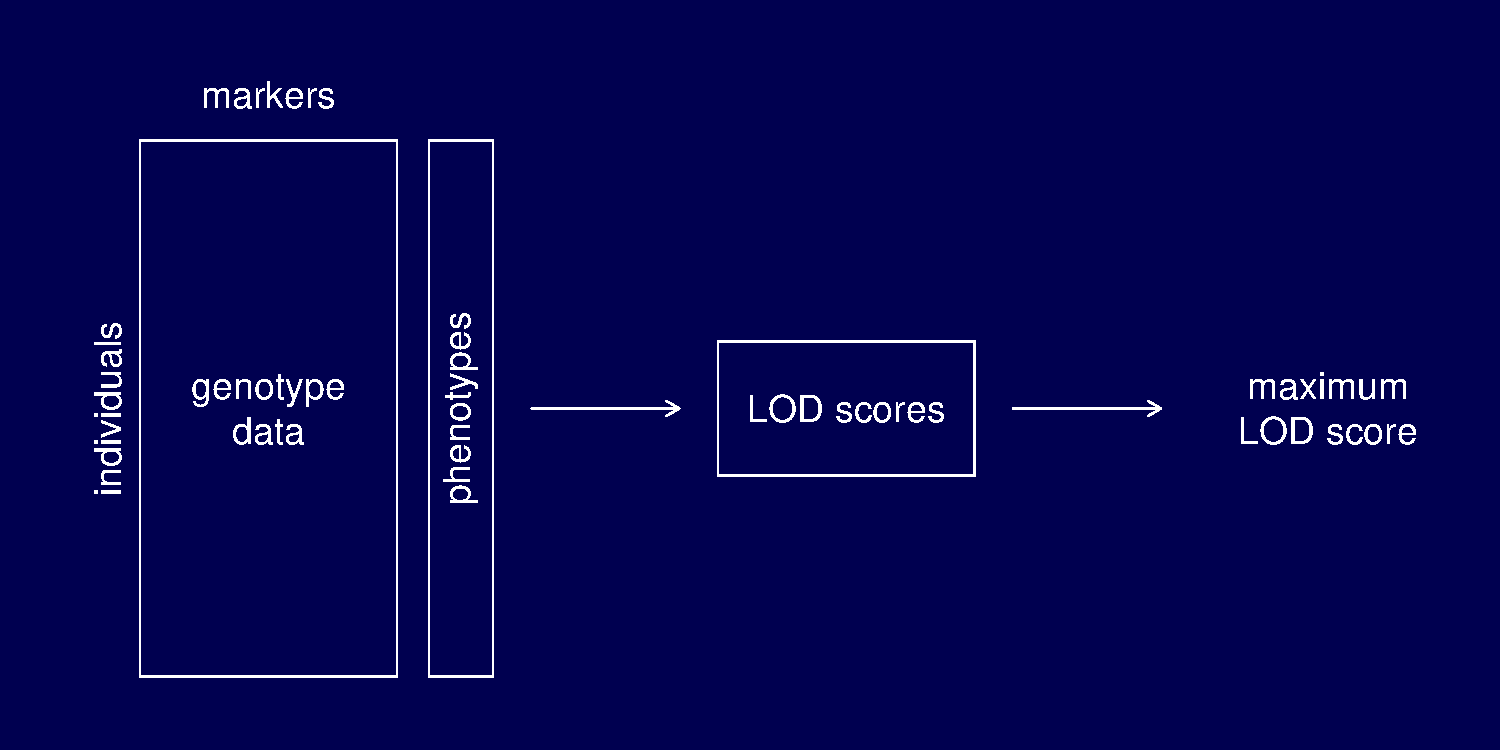
\includegraphics{FigsA/permtest.pdf}}

\newpage

\headsize \color{myyellow}
\hfill \begin{minipage}{5.75in}
\centering
Permutation results
\end{minipage}

\vfill

\centerline{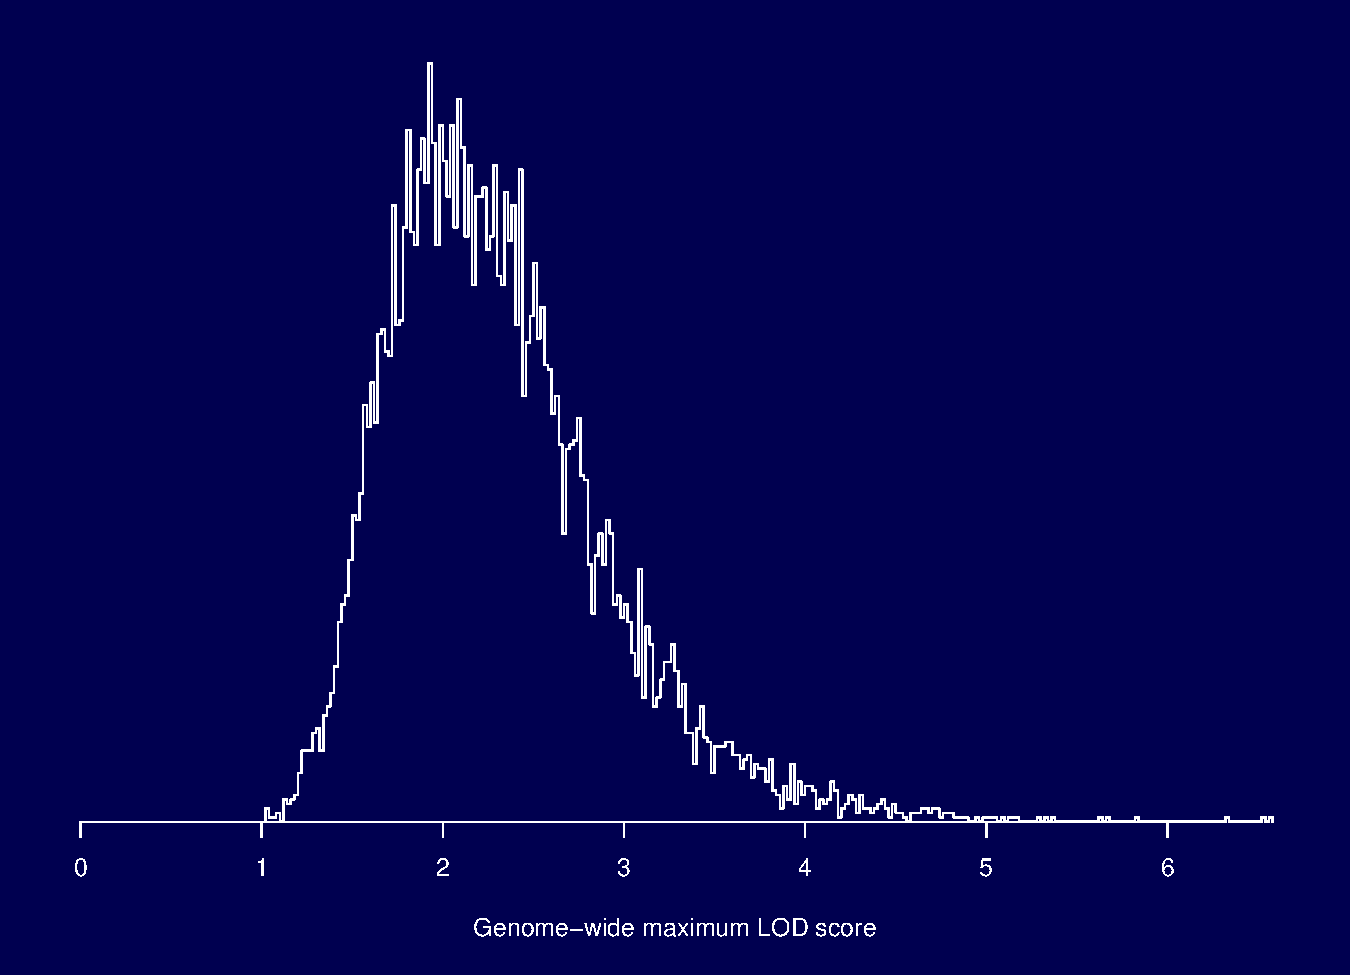
\includegraphics{FigsA/perm_hist.pdf}}



\newpage

\headsize \color{myyellow}
\hfill \begin{minipage}{5.75in}
\centering
\href{http://www.biostat.wisc.edu/~kbroman/D3/lod_random/}{Interactive plot}
\end{minipage}

\vspace{2cm}

\centerline{\href{http://www.biostat.wisc.edu/~kbroman/D3/lod_random}{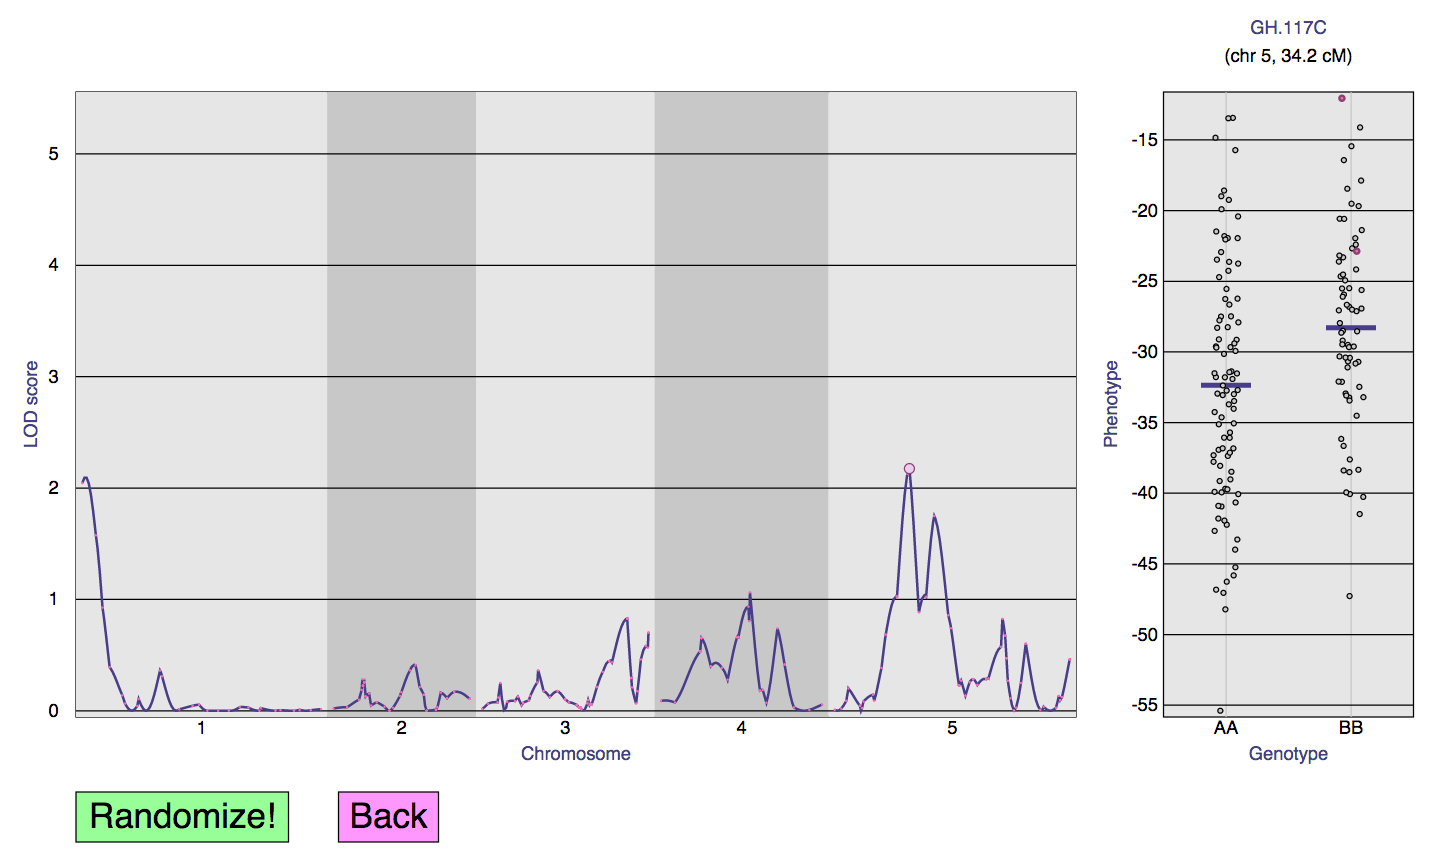
\includegraphics[width=10in]{FigsA/interactive_perm_test.png}}}

\vspace*{1cm}




\newpage

\headsize \color{myyellow}
$\boldsymbol{\rightarrow}$ R

\vspace{3cm}

\color{mywhite} \smallsize

\hfill \begin{minipage}[t]{9.5in}
\begin{itemize}
\itemsep24pt
\item \verb|scanone()| for permutations
\end{itemize} \end{minipage}








\newpage

\headsize \color{myyellow}
\hfill \begin{minipage}{5.75in}
\centering
LOD support intervals
\end{minipage}

\vfill

\centerline{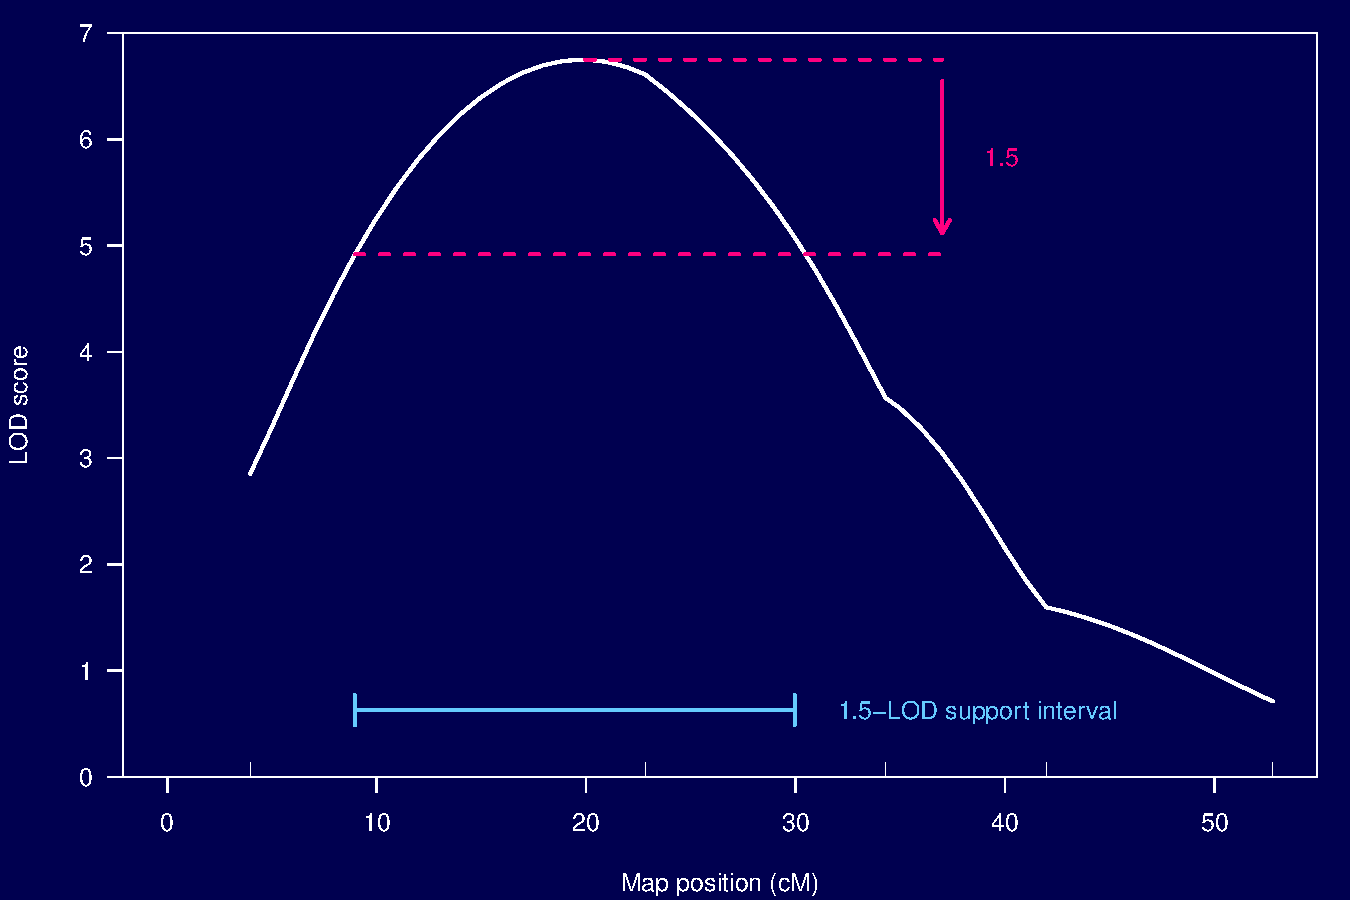
\includegraphics{FigsA/lodsuppint.pdf}}




\newpage

\headsize \color{myyellow}
$\boldsymbol{\rightarrow}$ R

\vspace{3cm}

\color{mywhite} \smallsize

\hfill \begin{minipage}[t]{9.5in}
\begin{itemize}
\itemsep24pt
\item \verb|lodint()|
\item \verb|bayesint()|
\end{itemize} \end{minipage}



\newpage

\headsize \color{myyellow}
\hfill \begin{minipage}{5.75in}
\centering
Haley-Knott regression
\end{minipage}

\vspace{3cm}

\color{mywhite} \smallsize

\hspace*{0.5in}
A quick approximation to Interval Mapping.

\smallersize

\begin{eqnarray*}
\mathsf{E(y_i | q_i)} & = & \mathsf{ \mu_q } \\[24pt]
\mathsf{E(y_i | M_i)} & = & \mathsf{E[ \ E(y_i|q_i) \ | M_i]}
 =  \mathsf{\textstyle{\sum_j \Pr(q=j|M_i) \mu_j}} \\[12pt]
& = & \mathsf{\textstyle{\sum_j p_{ij} \mu_j}}
\end{eqnarray*}

\vspace{1cm}

\hfill \begin{minipage}{10in}
\setlength{\rightskip}{0pt plus 1fil} % makes ragged right
{\color{mypink} Regress $\mathsf{y}$ on $\mathsf{p_i}$}, pretending the residual
variation is normally distributed (with constant variance).
\end{minipage}

\begin{eqnarray*}
\mathsf{\lod} & = & \mathsf{\frac{n}{2} \log_{10} \left( \frac{\rss_0}{\rss_1} \right)}
\end{eqnarray*}



\newpage

\headsize \color{myyellow}
$\boldsymbol{\rightarrow}$ R

\vspace{3cm}

\color{mywhite} \smallsize

\hfill \begin{minipage}[t]{9.5in}
\begin{itemize}
\itemsep24pt
\item \verb|scanone()| with \verb|method="hk"|
\end{itemize} \end{minipage}



\newpage

\headsize \color{myyellow}
\hfill \begin{minipage}{5.75in}
\centering
Haley-Knott results
\end{minipage}

\vfill

\centerline{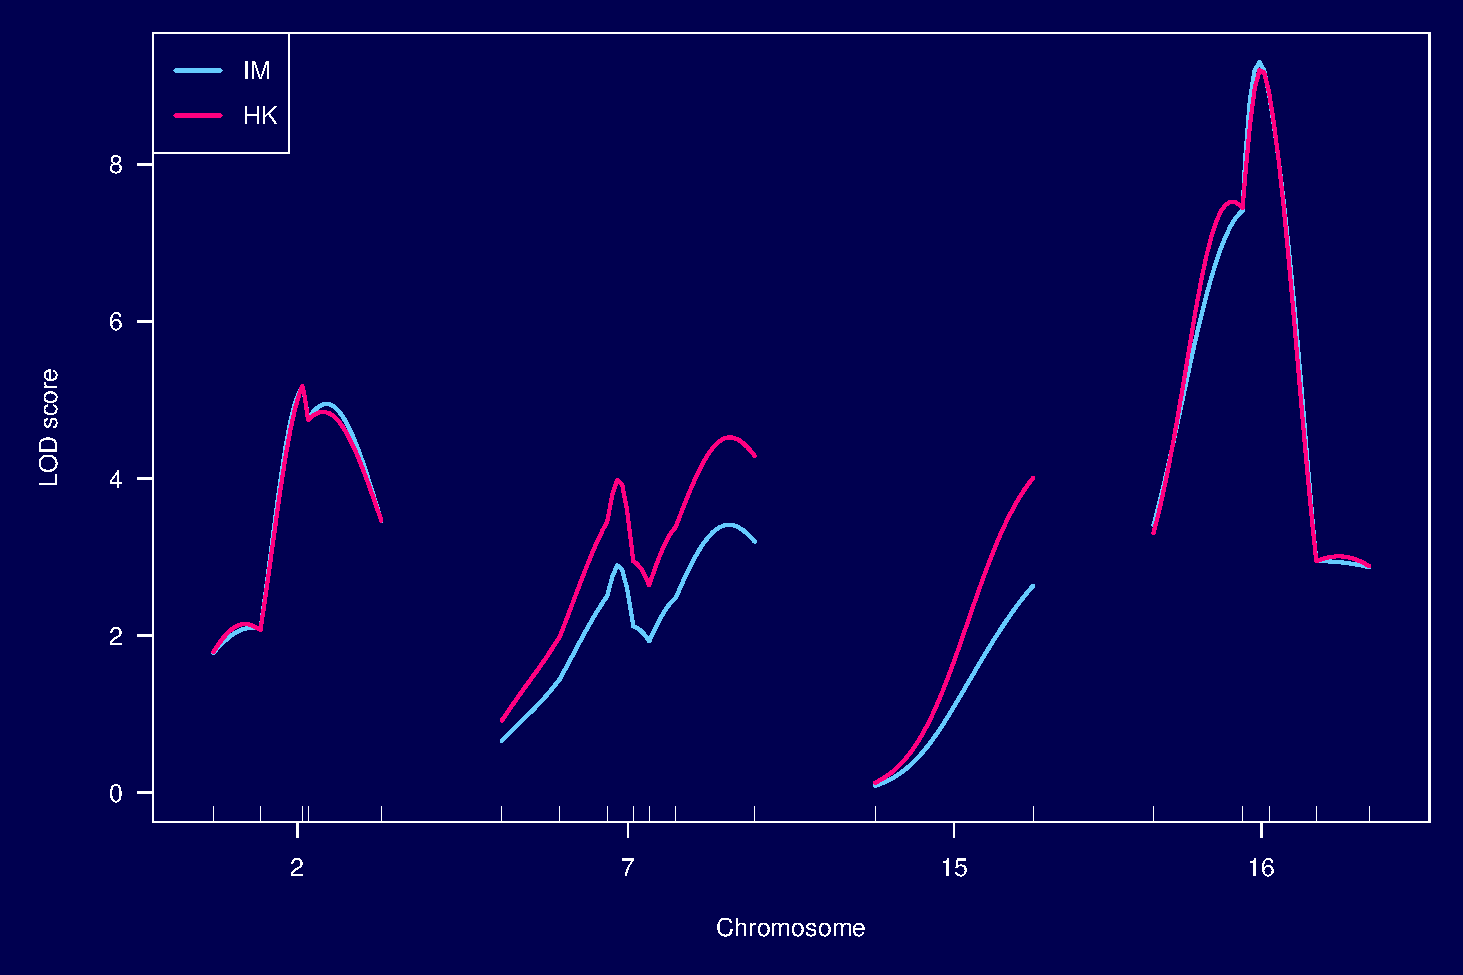
\includegraphics{FigsA/hk_lod.pdf}}



\newpage

\headsize \color{myyellow}
\hfill \begin{minipage}{5.75in}
\centering
H-K with selective genotyping
\end{minipage}

\vfill

\centerline{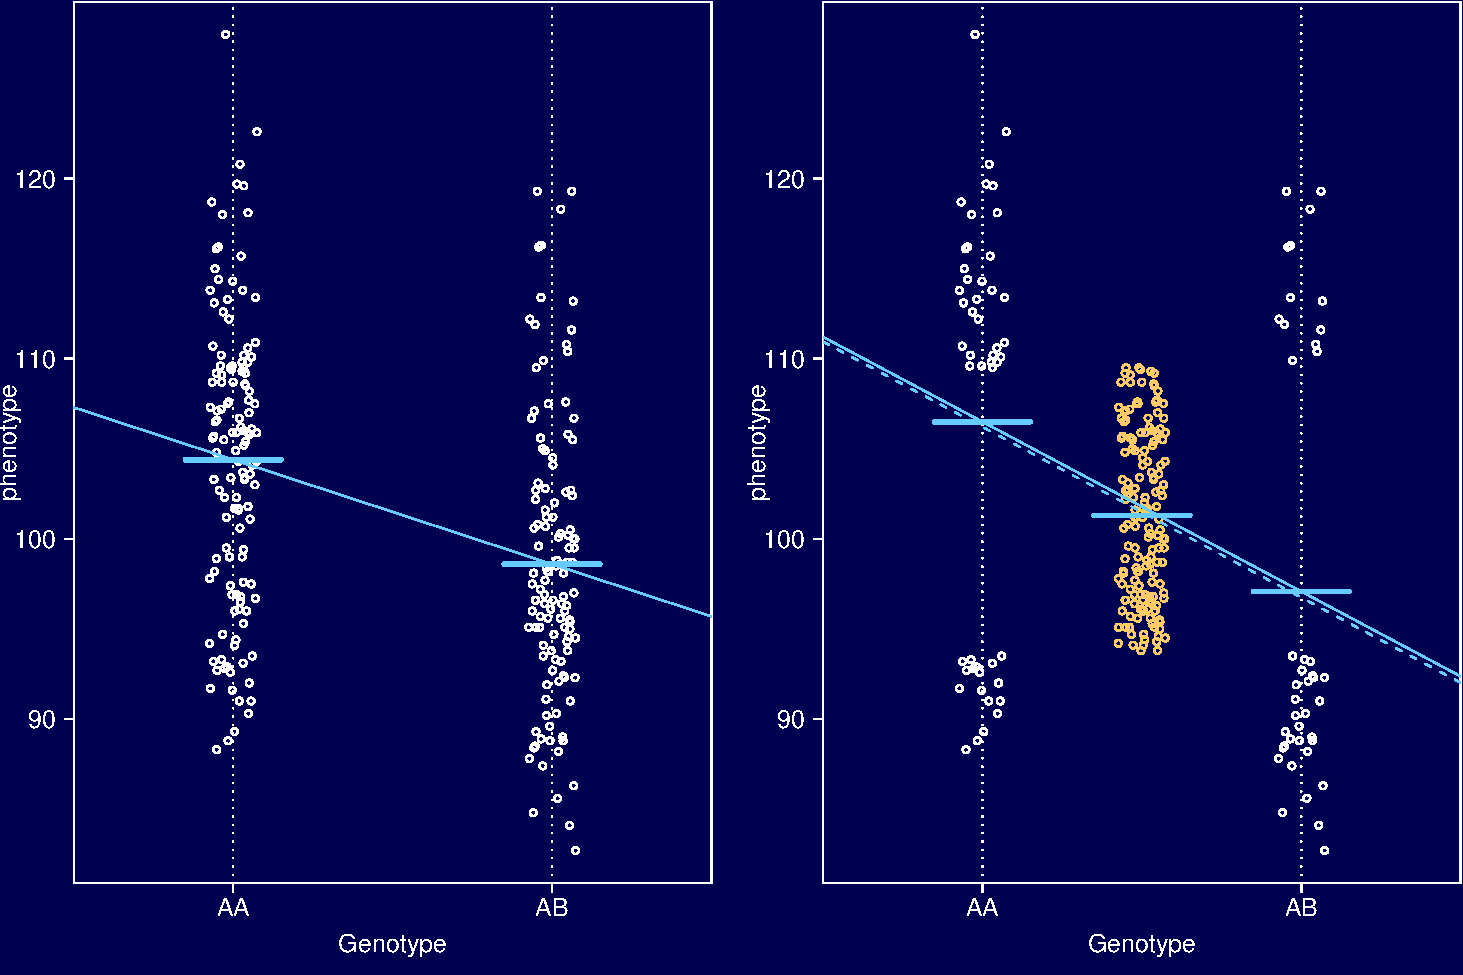
\includegraphics{FigsA/hk_selgeno.pdf}}





\newpage

\headsize \color{myyellow}
\hfill \begin{minipage}{5.75in}
\centering
Multiple imputation
\end{minipage}

\vfill

\centerline{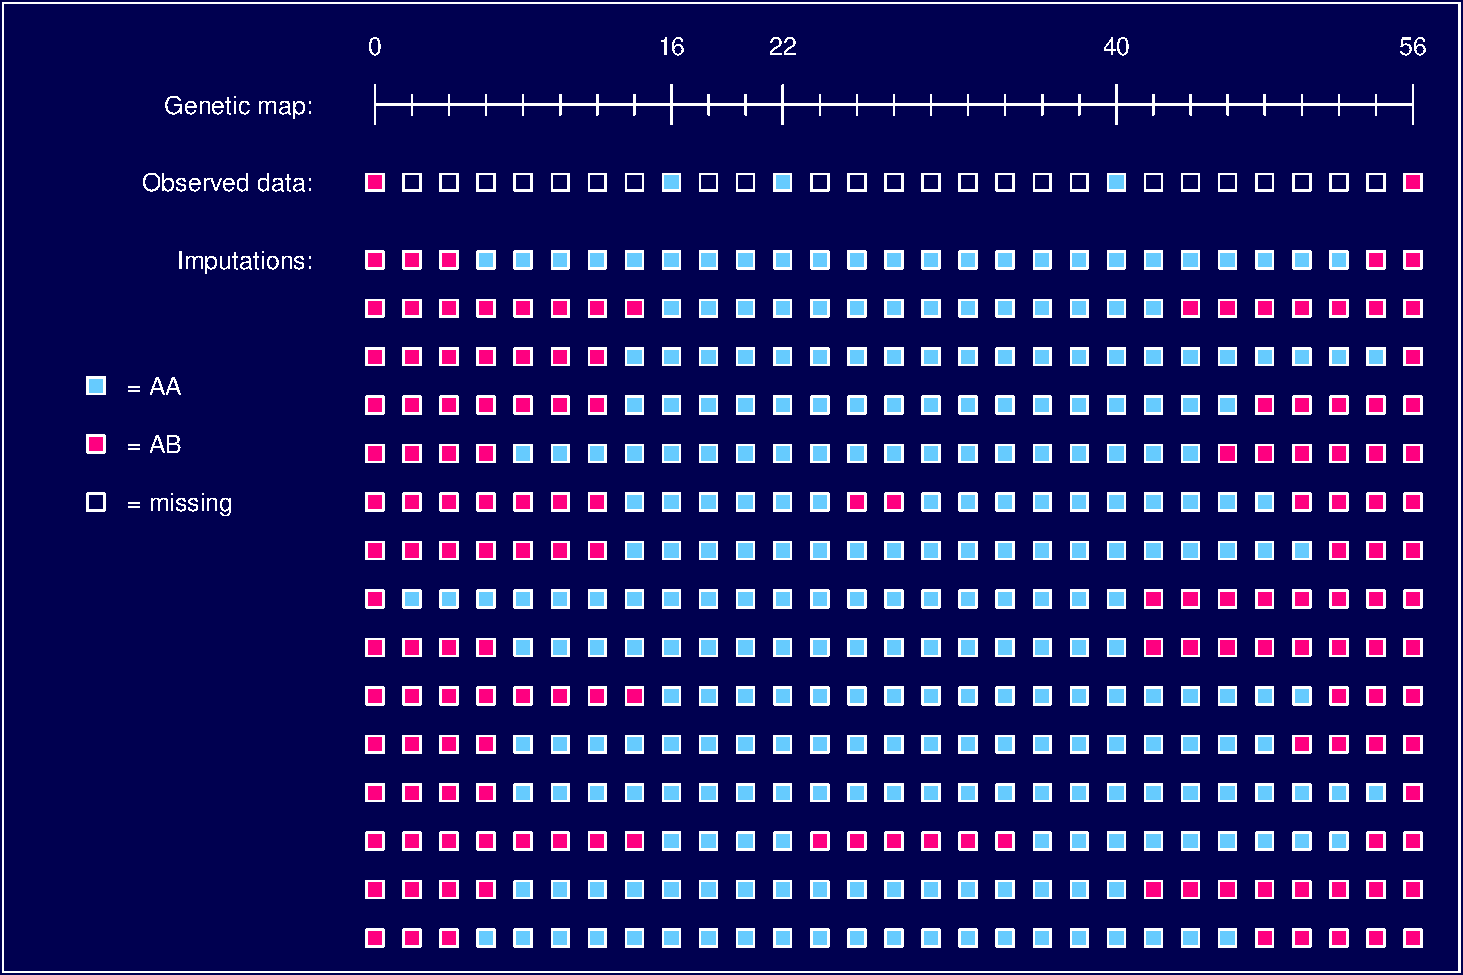
\includegraphics{FigsA/imp.pdf}}


\newpage

\headsize \color{myyellow}
\hfill \begin{minipage}{5.75in}
\centering
Multiple imputations
\end{minipage}

\vfill

\centerline{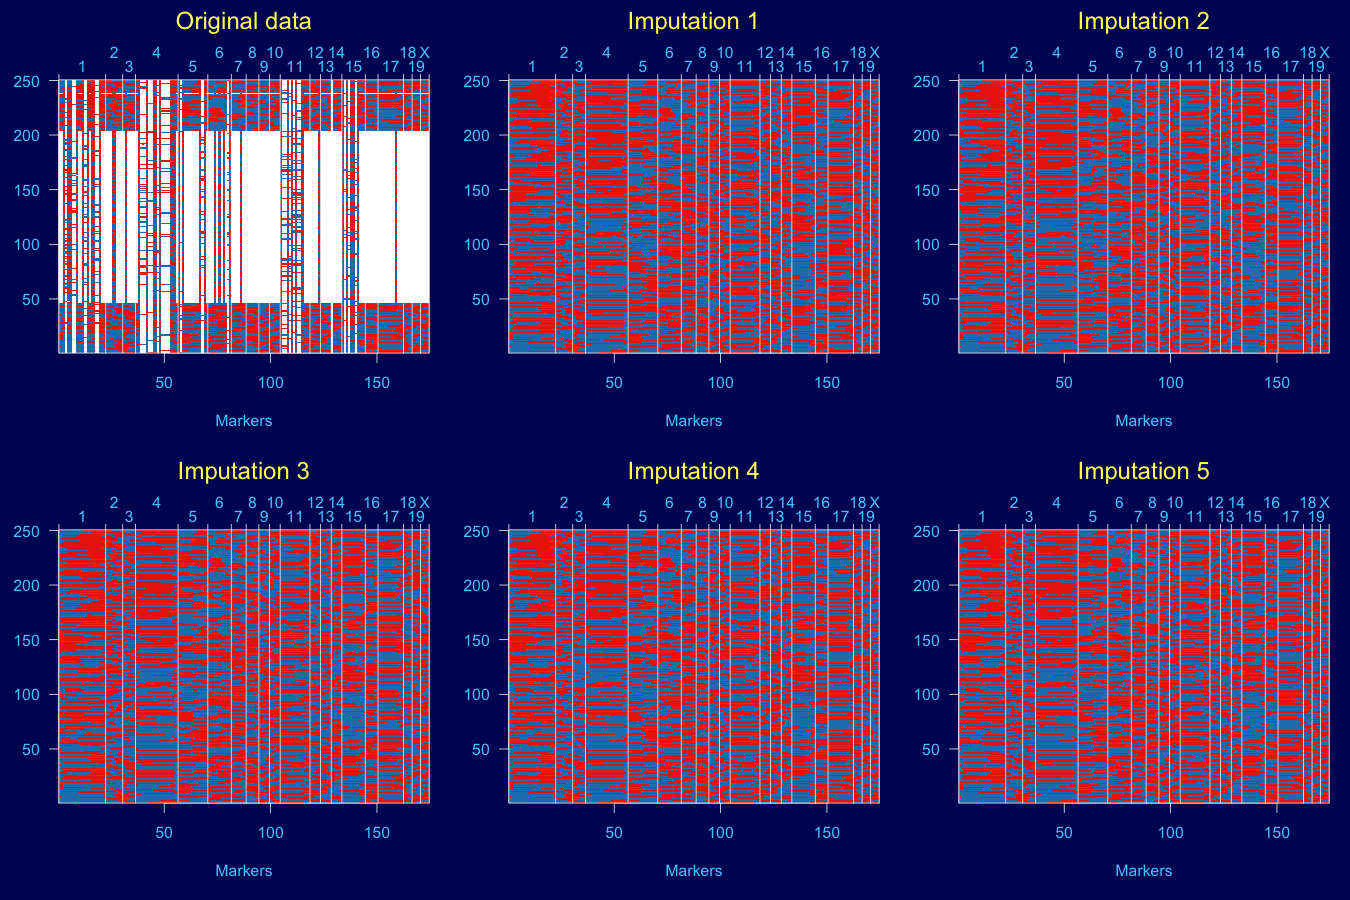
\includegraphics[height=6.5in]{FigsA/multiimp.png}}



\newpage

\headsize \color{myyellow}
\hfill \begin{minipage}{5.75in}
\centering
Imputation LOD curves
\end{minipage}

\vfill

\centerline{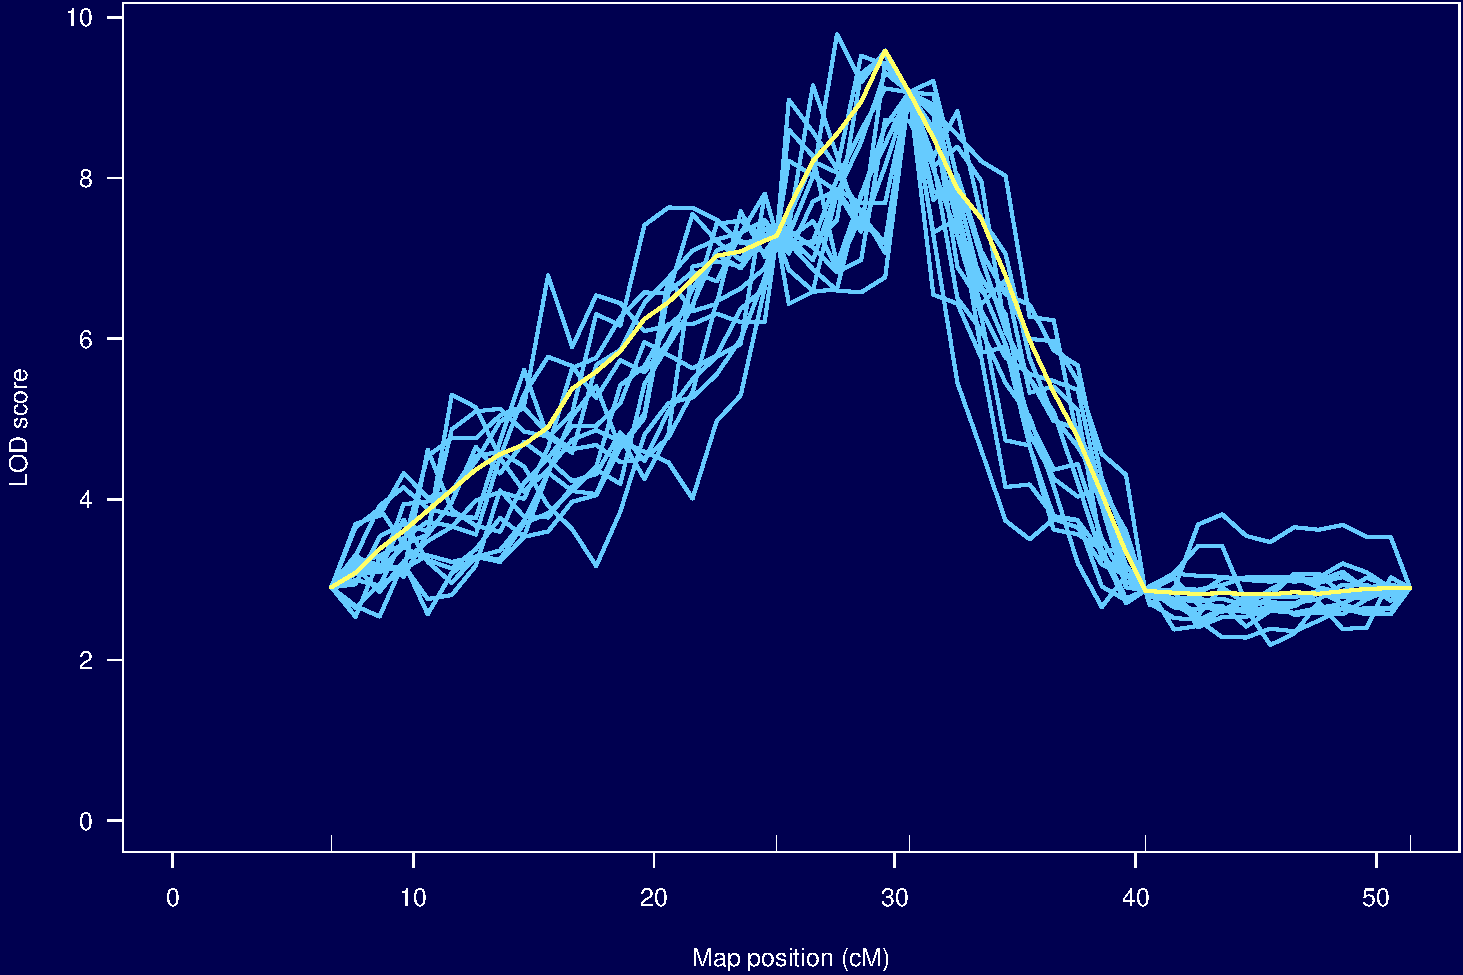
\includegraphics{FigsA/imp_lod.pdf}}




\newpage

\headsize \color{myyellow}
$\boldsymbol{\rightarrow}$ R

\vspace{3cm}

\color{mywhite} \smallsize

\hfill \begin{minipage}[t]{9.5in}
\begin{itemize}
\itemsep24pt
\item \verb|sim.geno()|
\item \verb|scanone()| with \verb|method="imp"|
\end{itemize} \end{minipage}




\newpage

\headsize \color{myyellow}
\hfill \begin{minipage}{5.75in}
\centering
Summary comparison
\end{minipage}


\vspace{25mm}

\begin{center}
\color{mywhite}
\smallersize

\renewcommand\arraystretch{2}
\begin{tabular}{cccccc}
\hline
Approach & Speed & Extensibility & Stability & Missing data &
Parallelization \\
\hline
HK & ++ & + & + & -- & ++ \\
EM & + & $-$ & $-$ & + & $-$ \\
Imputation & $-$ & + & + & + & + \\
\hline
\end{tabular}
\end{center}



\newpage

\headsize \color{myyellow}
\hfill \begin{minipage}{5.75in}
\centering
Non-normal traits
\end{minipage}


\vspace{25mm}

\color{mywhite} \smallersize
\hfill \begin{minipage}{10in}
\begin{itemize}
\setlength{\rightskip}{0pt plus 1fil} % makes ragged right
\itemsep18pt
\item Standard interval mapping assumes normally distributed residual
variation.  (Thus the phenotype distribution is a mixture of normals.)
\item {\color{mypink} In reality}: we see dichotomous traits,
counts, skewed distributions, outliers, and all sorts of odd things.
\item Interval mapping, with LOD thresholds derived from permutation
tests, generally performs just fine anyway.
\item Alternatives to consider:
\begin{itemize}
\smallersize
\setlength{\rightskip}{0pt plus 1fil} % makes ragged right
    \item Nonparametric approaches {\color{myblue} (Kruglyak \& Lander 1995)}
    \item Transformations {\color{myblue} (\emph{e.g.}, log, square root, normal quantiles)}
    \item Specially-tailored models  {\color{myblue} (\emph{e.g.}, a generalized linear
    model, the Cox proportional hazard model, and the two-part model
    in Broman 2003)}
\end{itemize}
\end{itemize} \end{minipage}




\newpage

\headsize \color{myyellow}
$\boldsymbol{\rightarrow}$ R

\vspace{3cm}

\color{mywhite} \smallsize

\hfill \begin{minipage}[t]{9.5in}
\begin{itemize}
\itemsep24pt
\item \verb|nqrank()|
\item \verb|scanone()| with \verb|model="binary"| or \verb|model="np"|
\end{itemize} \end{minipage}



\newpage

\headsize \color{myyellow}
\hfill \begin{minipage}{5.75in}
\centering
Covariates
\end{minipage}

\smallsize \color{mywhite}

\vspace{25mm}

\hfill
\begin{minipage}{10in}
\begin{itemize}
\setlength{\itemsep}{24pt}
\item {\color{mypink} Examples}: treatment, sex, age, weight

\item Control residual variation {\color{mypink} $\rightarrow$}
  increase power

\item Look for QTL $\times$ covariate interactions
\end{itemize}
\end{minipage}

\newpage

\headsize \color{myyellow}
\hfill \begin{minipage}{5.75in}
\centering
Additive covariate
\end{minipage}

\vspace{15mm}

\color{mywhite} \smallsize

\begin{eqnarray*}
\text{H}_0: y & = & \mu + \beta_x x + \epsilon \\
\text{H}_a: y & = & \mu + \beta_x x + \beta_q q + \epsilon
\end{eqnarray*}

\vspace{30mm}

\hspace{0.5in}
\begin{minipage}{9.5in}
\begin{itemize}
\itemsep20pt
\item If covariate has strong effect on the phenotype, accounting for
  it can give improved power to detect QTL.
\item In permutations, keep phenotype and covariate together
\item Use care when the covariate is another phenotype
\end{itemize}
\end{minipage}

\newpage

\headsize \color{myyellow}
\hfill \begin{minipage}{5.75in}
\centering
Additive covariate
\end{minipage}

\vfill

\centerline{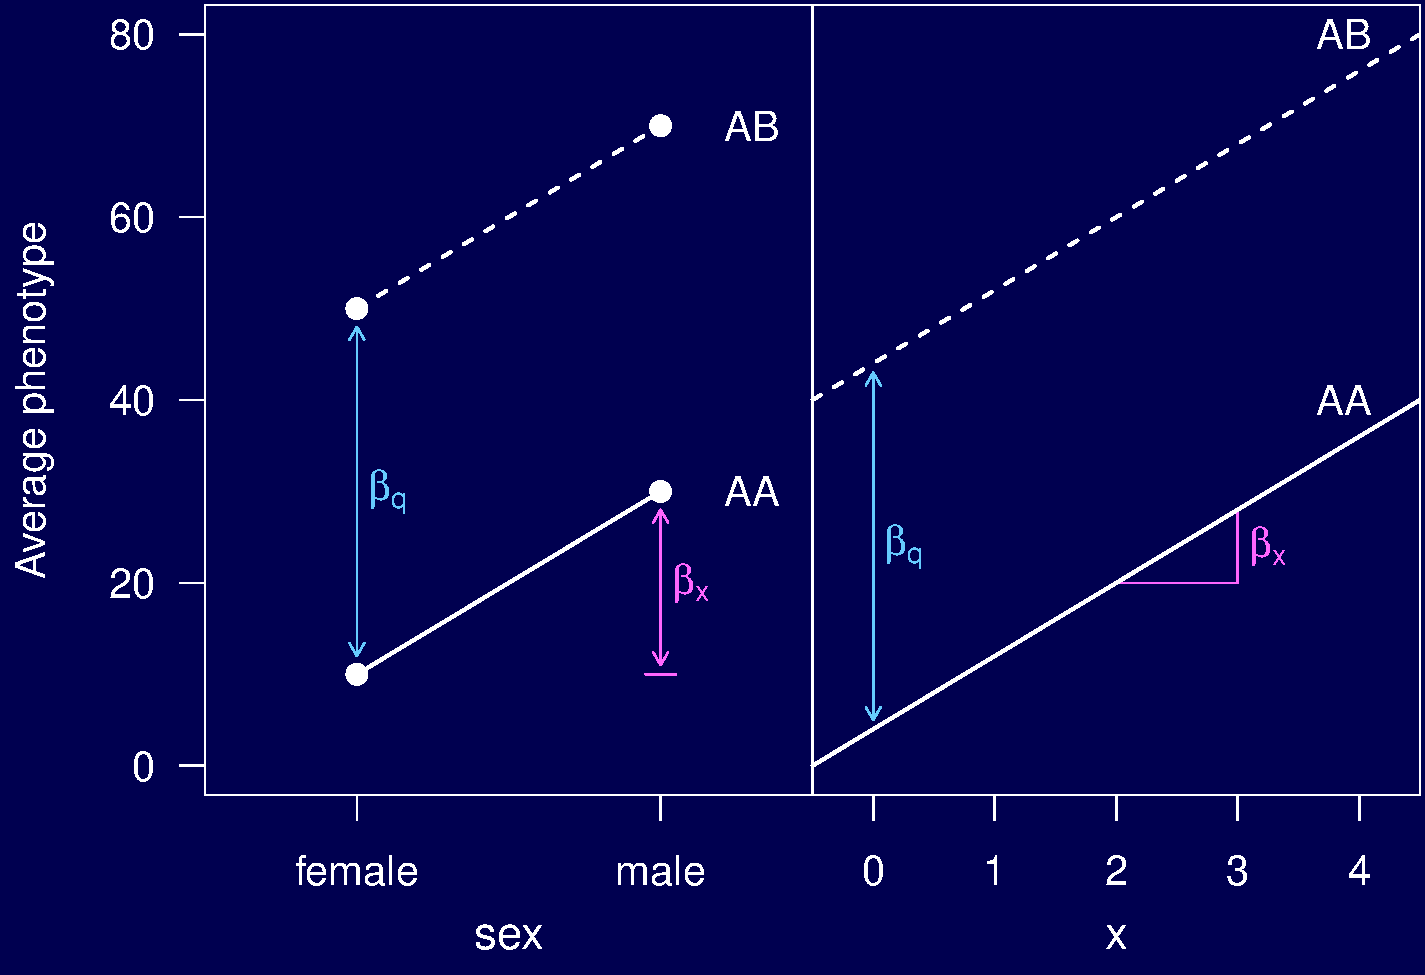
\includegraphics{FigsA/addcovar.pdf}}

\newpage

\headsize \color{myyellow}
\hfill \begin{minipage}{5.75in}
\centering
Adjust then scan?
\end{minipage}

\vspace{15mm}

\color{mywhite} \smallsize

\hspace{0.5in} \begin{minipage}{9.5in}
  \begin{itemize}
    \itemsep18pt
  \item Consider adjusted phenotype $y' = y/x$
  \item The QTL model is $(y/x) = \mu + \beta_q q + \epsilon$
  \item Equivalently

$$y = \left\{ \begin{array}{c@{\hspace{1cm}}l} \mu \ x + \epsilon' & \text{if
      $q = 0$} \\
    (\mu + \beta_q) x + \epsilon' & \text{if $q =
      1$} \end{array} \right. $$
\end{itemize}
\end{minipage}


\newpage

\headsize \color{myyellow}
\hfill \begin{minipage}{5.75in}
\centering
Adjust then scan?
\end{minipage}

\vfill

\centerline{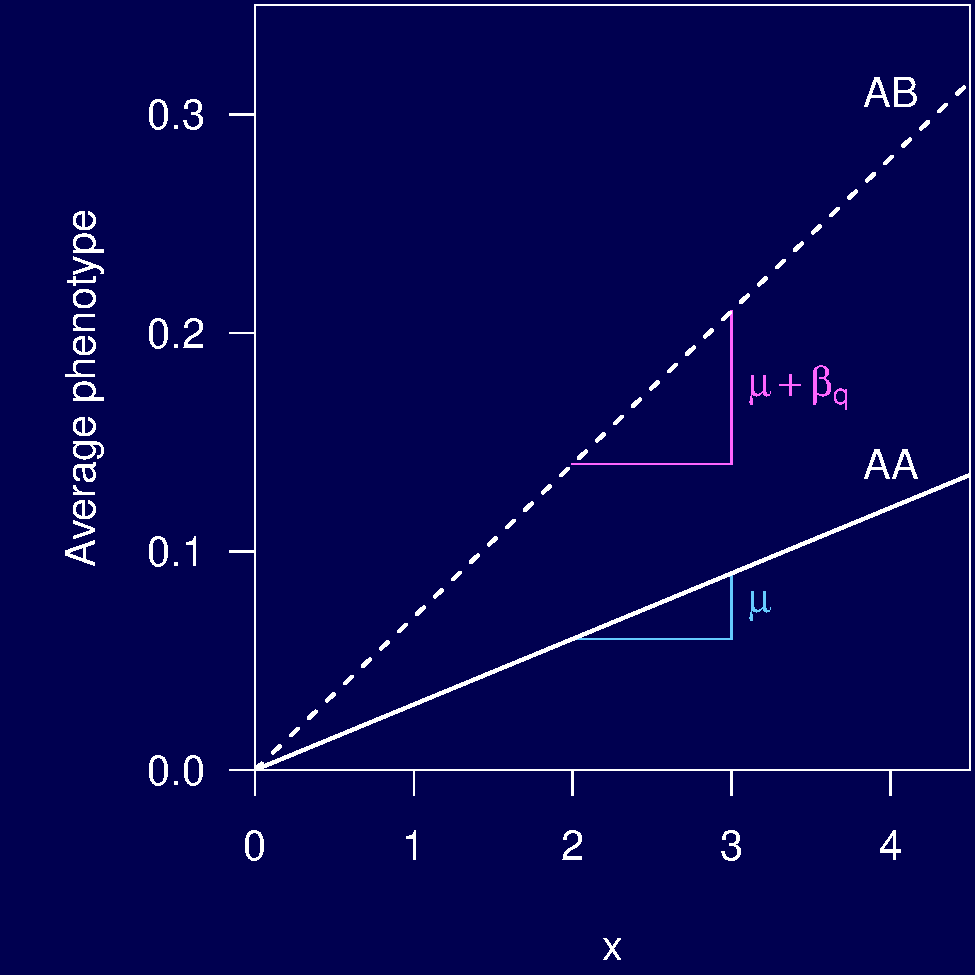
\includegraphics{FigsA/y_over_x.pdf}}




\newpage

\headsize \color{myyellow}
\hfill \begin{minipage}{5.75in}
\centering
Interactive covariate
\end{minipage}

\vspace{15mm}

\color{mywhite} \smallsize

\begin{eqnarray*}
\text{H}_0: y & = & \mu + \beta_x x + \epsilon \\
\text{H}_a: y & = & \mu + \beta_x x + \beta_q q + \epsilon \\
\text{H}_i: y & = & \mu + \beta_x x + \beta_q q + \gamma x q + \epsilon
\end{eqnarray*}

\vspace{15mm}

\hspace{0.5in}
\begin{minipage}{9.5in}
Can consider 3 LOD scores:
  \begin{itemize}
    \item LOD$_a$ comparing H$_a$ and H$_0$
    \item LOD$_f$ comparing H$_i$ and H$_0$
    \item LOD$_i$ comparing H$_i$ and H$_a$
  \end{itemize}
\end{minipage}

\newpage

\headsize \color{myyellow}
\hfill \begin{minipage}{5.75in}
\centering
Interactive covariate
\end{minipage}

\vfill

\centerline{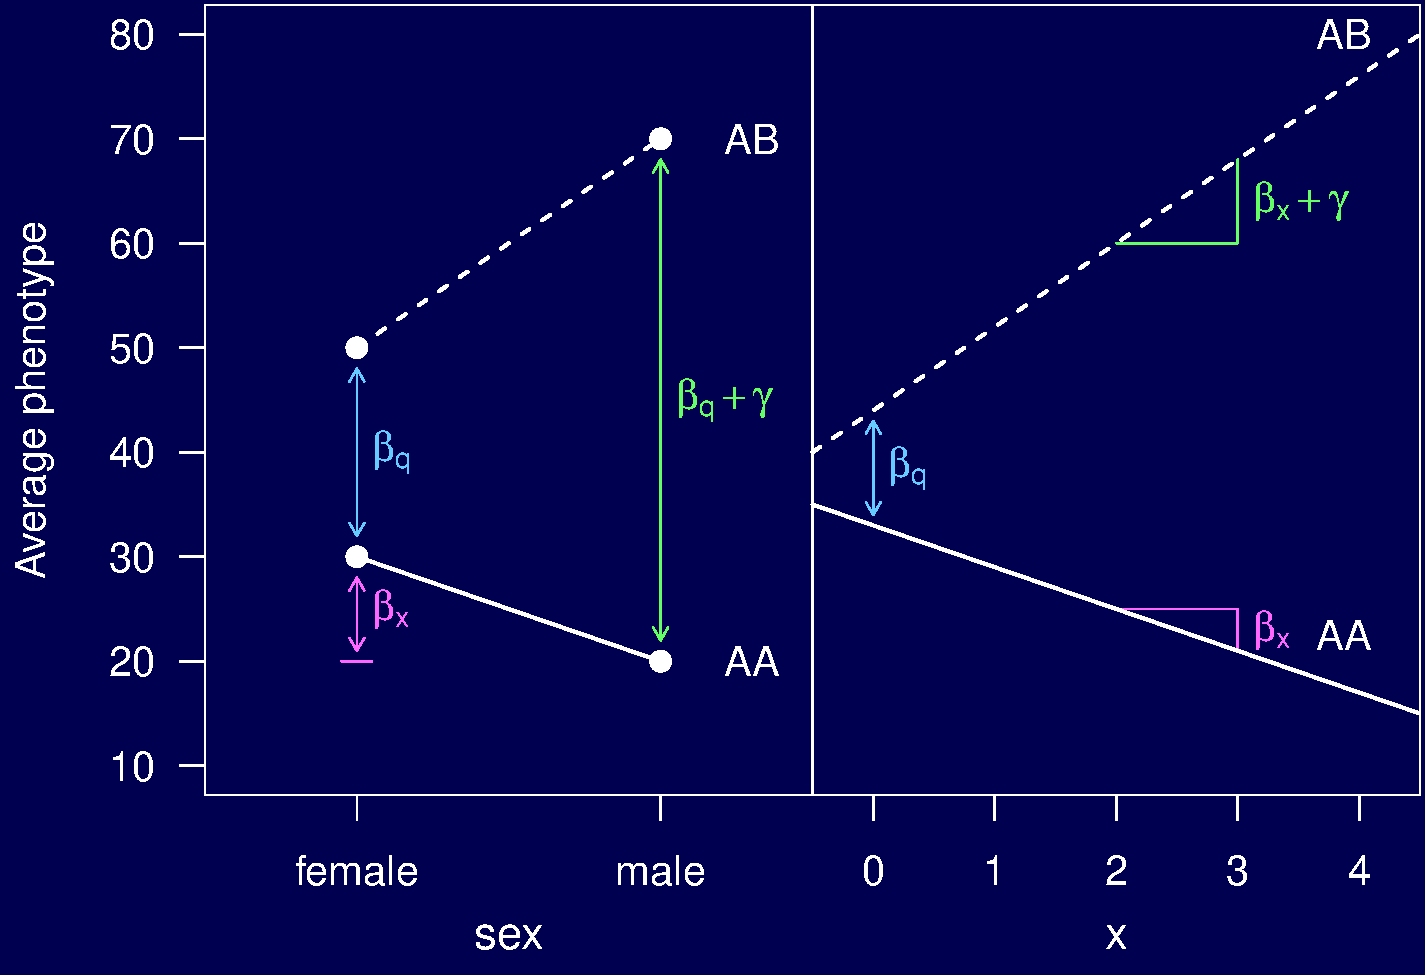
\includegraphics{FigsA/intcovar.pdf}}


\newpage

\headsize \color{myyellow}
\hfill \begin{minipage}{5.75in}
\centering
Split on sex?
\end{minipage}

\vspace{15mm}

\color{mywhite} \smallsize

\hspace*{0.5in}
\begin{minipage}[t]{4.1in}
\vspace*{25mm}

\sloppy
\smallersize
\begin{itemize}
\setlength{\rightskip}{0pt plus 1fil} % makes ragged right
\item Informative, understandable
\item But tempting to falsely conclude
  ``{\color{mypink} sex-specific QTL}''
\item Absence of evidence {\color{mypink} is not}
  \emph{evidence of absence}.
\item Use explicit test of QTL $\times$ sex interaction
\end{itemize}
\end{minipage}
\hfill
\begin{minipage}[t]{5.3in}
\vspace*{0mm}

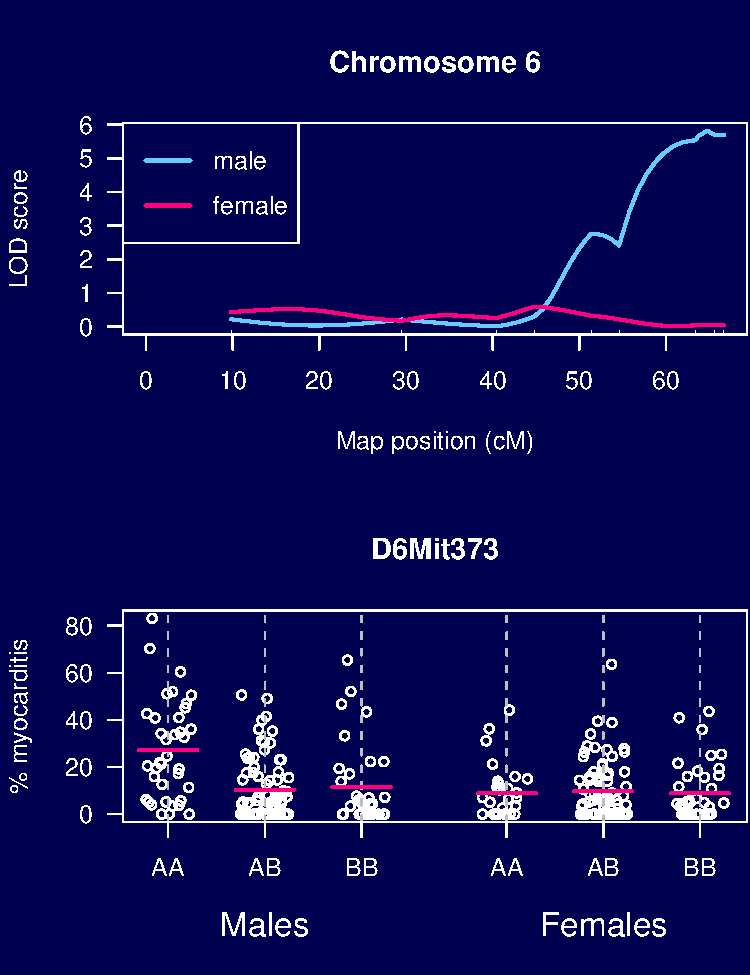
\includegraphics{FigsA/covar.pdf}
\end{minipage}


\newpage

\headsize \color{myyellow}
$\boldsymbol{\rightarrow}$ R

\vspace{3cm}

\color{mywhite} \smallsize

\hfill \begin{minipage}[t]{9.5in}
\begin{itemize}
\itemsep24pt
\item \verb|scanone()| with \verb|addcovar| and \verb|intcovar|
\item \verb|set.seed()| to do permutations
\item \verb|subset()| to split on sex
\end{itemize} \end{minipage}


\newpage

\headsize \color{myyellow}
\hfill \begin{minipage}{5.75in}
\centering
X chr in backcross
\end{minipage}

\vfill

\centerline{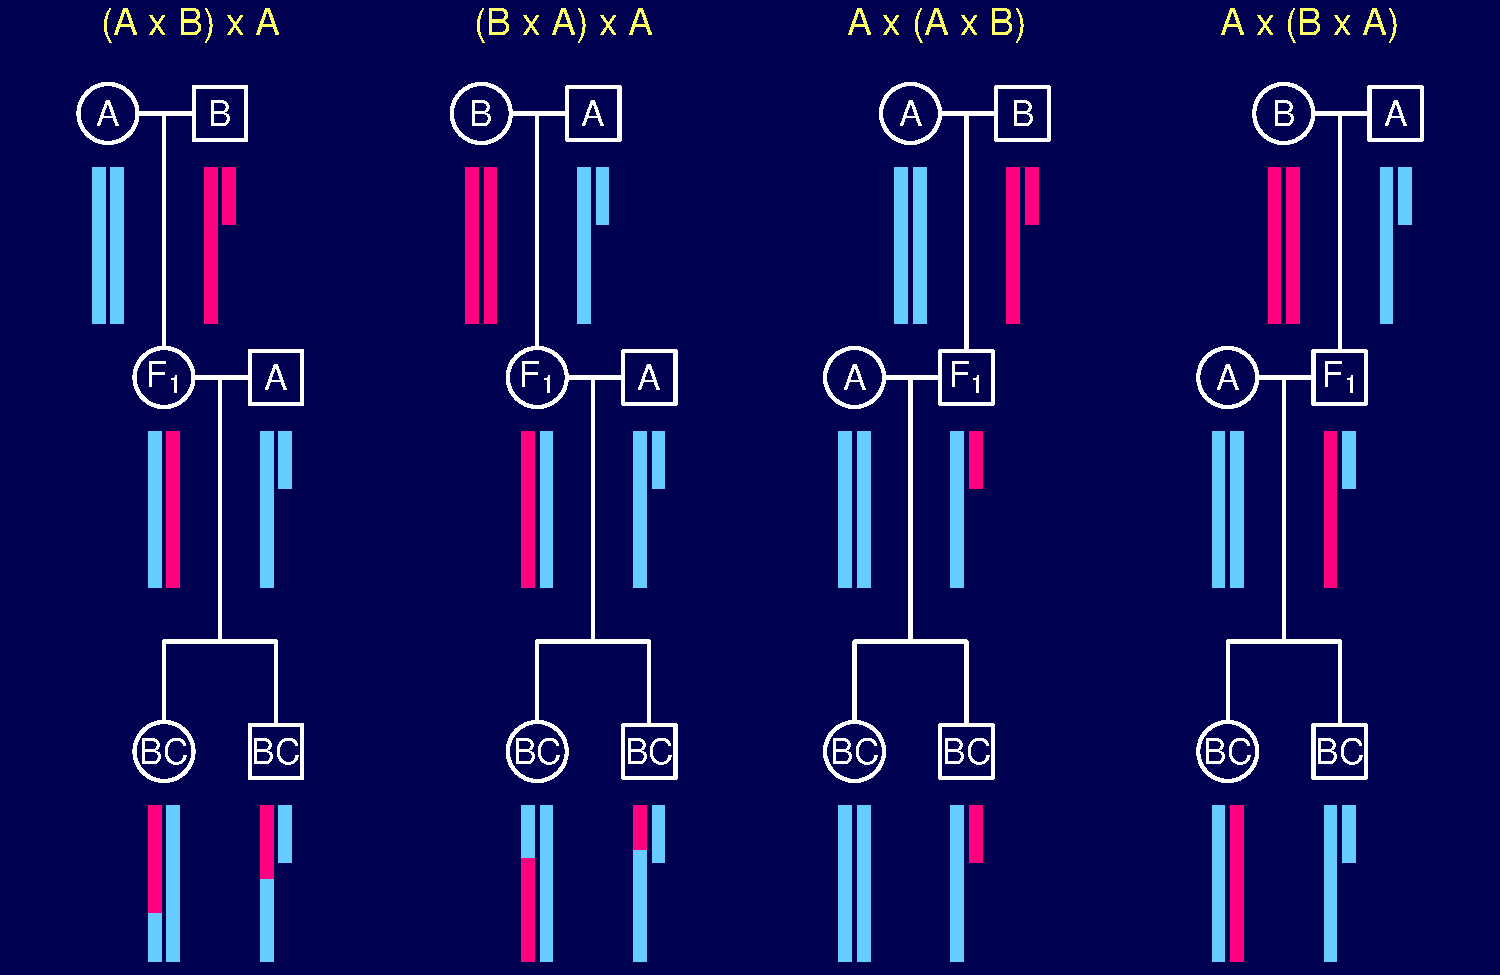
\includegraphics[]{FigsA/xchr_bc.pdf}}


\newpage

\headsize \color{myyellow}
\hfill \begin{minipage}{5.75in}
\centering
X chr in intercross
\end{minipage}

\vfill

\centerline{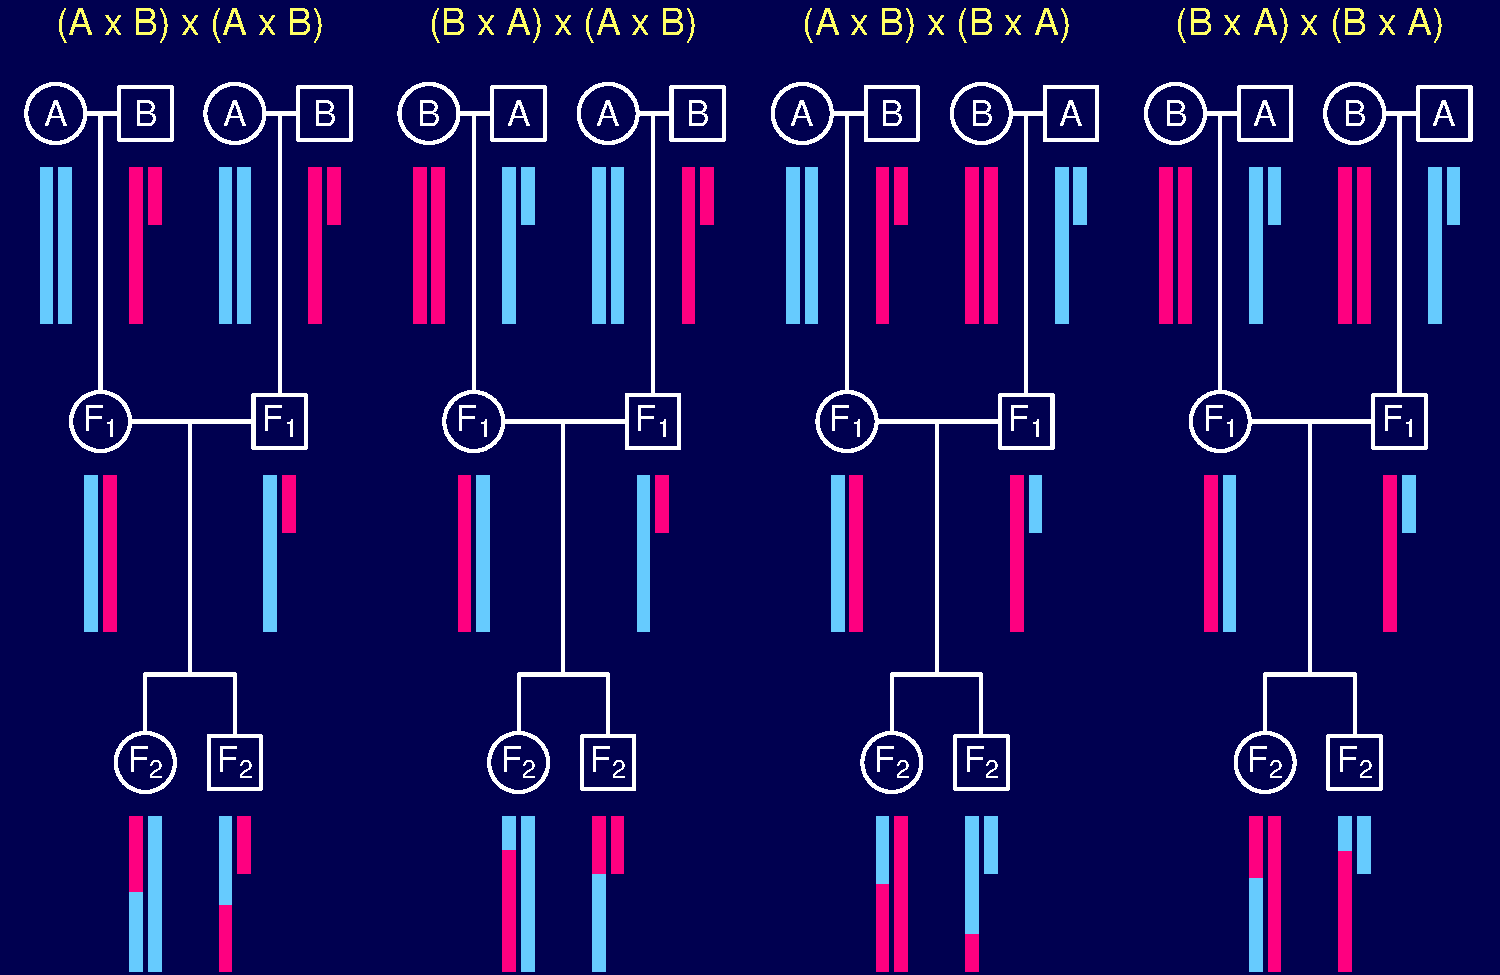
\includegraphics[]{FigsA/xchr_f2.pdf}}


\newpage

\headsize \color{myyellow}
\hfill \begin{minipage}{5.75in}
\centering
Example
\end{minipage}

\vspace{3cm}

\color{mywhite} \textsize

\hspace{0.5in} \begin{minipage}{9.5in}

Intercross: both dir, both sexes

\vspace{20mm}

\color{myblue} \smallsize

\hspace*{1in} \begin{tabular}{cccccccccccc}
{\textsize \female} & forward & \hspace{1cm} & AA & or & AB \\[18pt]
{\textsize \female} & reverse &              &    &    & AB & or & BB \\[18pt]
{\textsize   \male} & forward &            &    &    &    &    &    & AY & or & BY \\[18pt]
{\textsize   \male} & reverse &              &    &    &    &    &    & AY & or & BY
\end{tabular}
\end{minipage}


\newpage

\headsize \color{myyellow}
$\boldsymbol{\rightarrow}$ R

\vspace{3cm}

\color{mywhite} \smallsize

\hfill \begin{minipage}[t]{9.5in}
\begin{itemize}
\itemsep24pt
\item \verb|scanone()| permutations with \verb|perm.Xsp=TRUE|
\end{itemize} \end{minipage}




\newpage

\headsize \color{myyellow}
\hfill \begin{minipage}{5.75in}
\centering
Data diagnostics
\end{minipage}

\vspace{3cm}

\color{mywhite} \smallsize

\hfill \begin{minipage}[t]{9.5in}
\begin{itemize}
\itemsep18pt
\item Plot phenotypes
\item Look for sample duplicates
\item Look for excessive missing data
\item Investigate segregation distortion
\item Verify genetic maps/marker positions
\item Look for genotyping errors
\item Look at counts of crossovers
\end{itemize} \end{minipage}

\vspace{15mm}

\centerline{\color{myblue} See Ch 3 in the R/qtl book,
  \href{http://rqtl.org/book}{\tt rqtl.org/book}}


\newpage

\headsize \color{myyellow}
\hfill \begin{minipage}{5.75in}
\centering
Modeling multiple QTL
\end{minipage}

\vspace{3cm}

\color{mywhite} \smallsize

\hfill \begin{minipage}[t]{10in}
\begin{itemize}
\itemsep24pt
\item Reduce residual variation $\longrightarrow$ increased power

\item Separate linked QTL

\item Identify interactions among QTL {\color{myblue} (epistasis)}

\end{itemize}
\end{minipage}


\newpage

\headsize \color{myyellow}
\hfill \begin{minipage}{5.75in}
\centering
Epistasis in BC
\end{minipage}

\vfill

\centerline{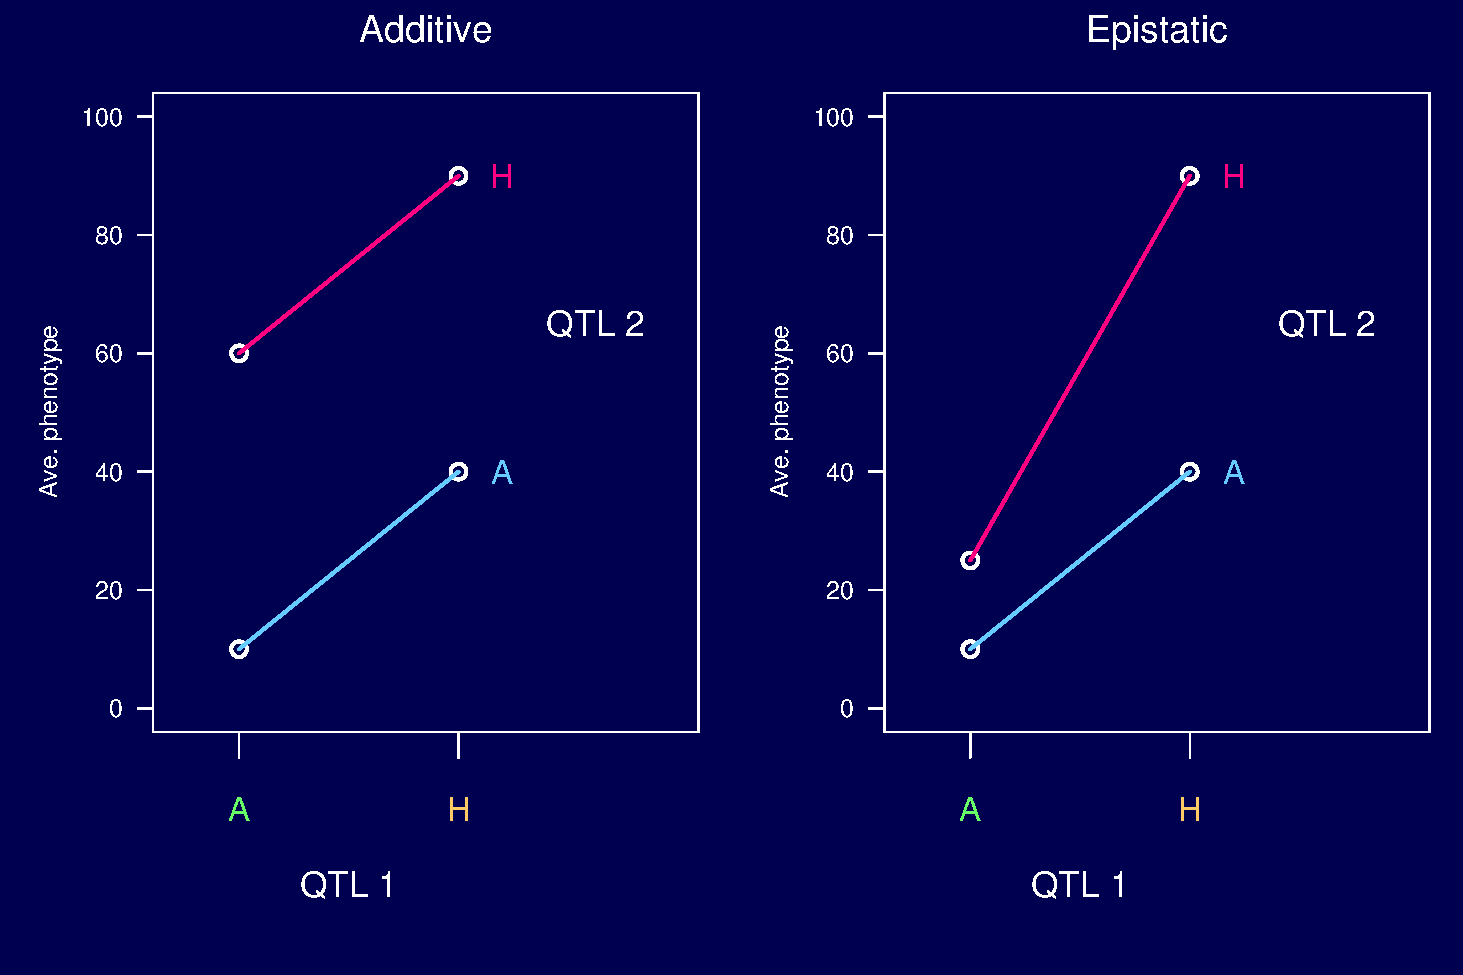
\includegraphics{FigsB/epistasis_bc.pdf}}


\newpage

\headsize \color{myyellow}
\hfill \begin{minipage}{5.75in}
\centering
Epistasis in F$_{\mathsf{2}}$
\end{minipage}

\vfill

\centerline{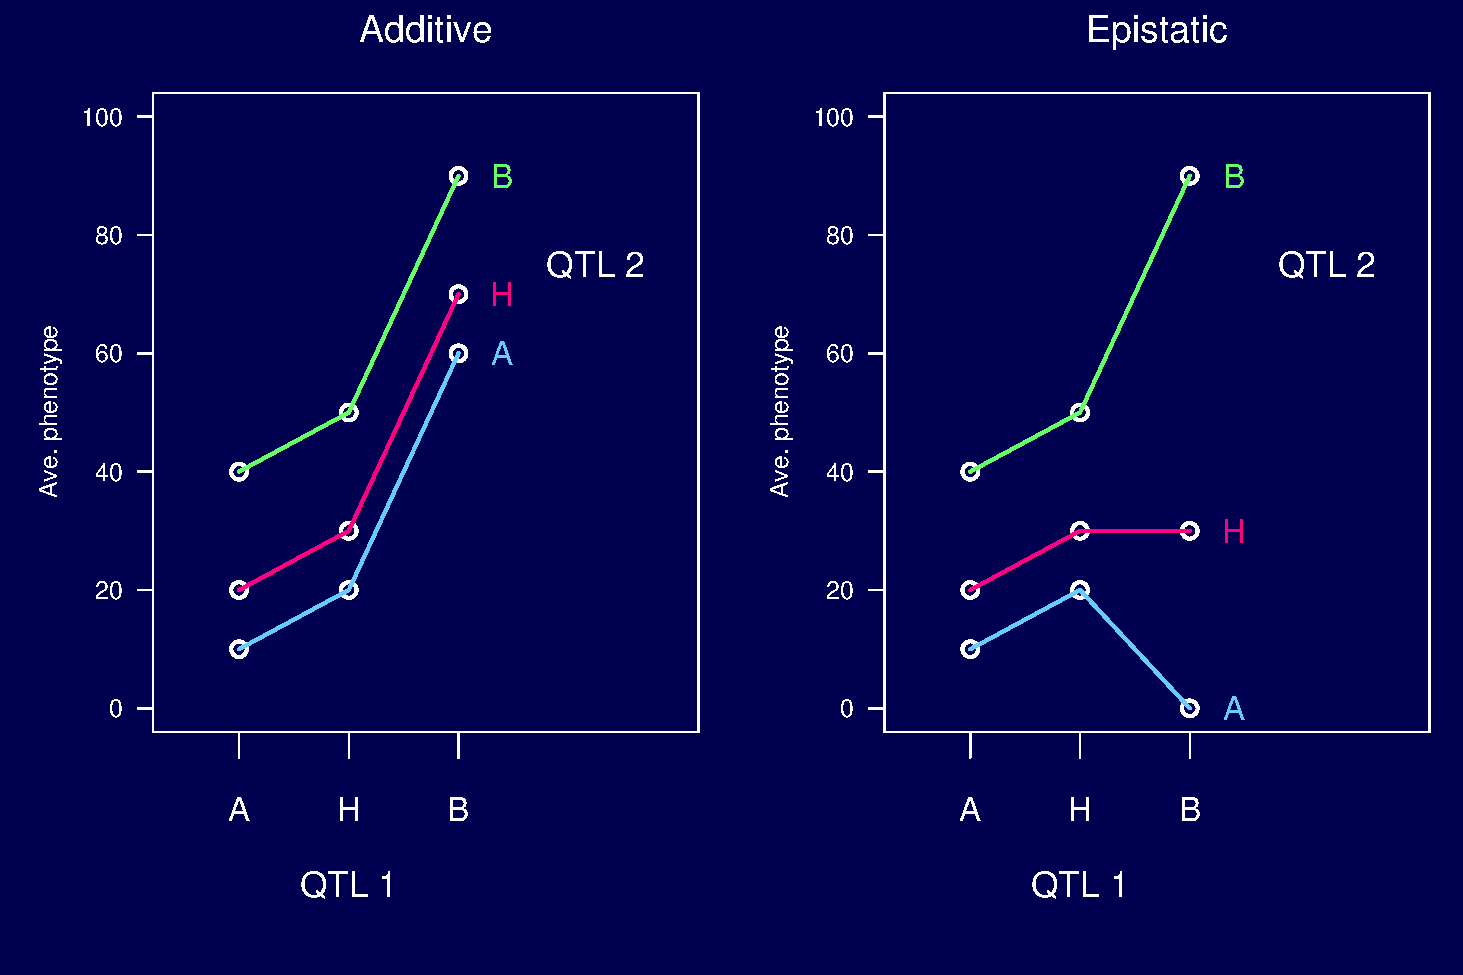
\includegraphics{FigsB/epistasis_f2.pdf}}



\newpage

\headsize \color{myyellow}
\hfill \begin{minipage}{5.75in}
\centering
2-dim, 2-QTL scan
\end{minipage}

\vspace{2cm}

\color{mywhite} \smallsize

\hfill \begin{minipage}[t]{10in}
For all pairs of positions, fit the following models:

\vspace{10mm}

\hfill
\begin{minipage}{9in}
{\color{myblue}
$\mathsf{\text{H}_f: y = \mu + \beta_1 q_1 + \beta_2 q_2 +
      \gamma q_1 q_2 + \epsilon}$

\vspace{5mm}

$\mathsf{\text{H}_a: y = \mu + \beta_1 q_1 + \beta_2 q_2 +
      + \epsilon}$

\vspace{5mm}

$\mathsf{\text{H}_1: y = \mu + \beta_1 q_1 + \epsilon}$

\vspace{5mm}

$\mathsf{\text{H}_0: y = \mu + \epsilon}$

}
\end{minipage}

\vspace{20mm}

log$_{\mathsf{10}}$ likelihoods:

\vspace{5mm}

\hfill
\begin{minipage}{9in}
{\color{myblue}

$\mathsf{l_f(s,t)}$ \hspace{2cm}
$\mathsf{l_a(s,t)}$ \hspace{2cm}
$\mathsf{l_1(s)}$ \hspace{2cm}
$\mathsf{l_0}$ \hspace{2cm}
}
\end{minipage}


\end{minipage}


\newpage

\headsize \color{myyellow}
\hfill \begin{minipage}{5.75in}
\centering
2-dim, 2-QTL scan
\end{minipage}

\vspace{2cm}

\color{mywhite} \smallsize

\hfill \begin{minipage}[t]{10in}
LOD scores:

\vspace{5mm}

\hspace{1cm}
\begin{minipage}{5in}
{\color{myblue}
\begin{eqnarray*}
\mathsf{\lod_f(s,t)}& = &\mathsf{l_f(s,t) - l_0} \\[24pt]
\mathsf{\lod_a(s,t)}& = &\mathsf{l_a(s,t) - l_0} \\[24pt]
\mathsf{\lod_i(s,t)}& = &\mathsf{l_f(s,t) - l_a(s,t)} \\[24pt]
\mathsf{\lod_1(s)}&   = &\mathsf{l_1(s) - l_0} \\[24pt]
\end{eqnarray*}
}
\end{minipage}



\end{minipage}


\newpage

\headsize \color{myyellow}
\hfill \begin{minipage}{5.75in}
\centering
Summaries
\end{minipage}

\vspace{15mm}

\color{mywhite} \smallsize

\hfill \begin{minipage}[t]{10in}
Consider each pair of chromosomes, {\color{myblue} $\mathsf{(j, k)}$}, \\
and let {\color{myblue} $\mathsf{c(s)}$} denote the chromosome for
  position {\color{myblue} $\mathsf{s}$}.

\vspace{5mm}

\hspace{1in}
\begin{minipage}{6in}
{\color{myblue}
\begin{eqnarray*}
\mathsf{\M_f(j,k)}& = &\mathsf{ \max_{c(s)=j, c(t)=k} \lod_f(s,t)} \\[12pt]
\mathsf{\M_a(j,k)}& = &\mathsf{ \max_{c(s)=j, c(t)=k} \lod_a(s,t)} \\[12pt]
\mathsf{\M_1(j,k)}& = &\mathsf{ \max_{c(s)=j \text{ or } k} \lod_1(s)} \\[36pt]
\mathsf{\M_i(j,k)}& = &\mathsf{ \M_f(j,k) - \M_a(j,k)}\\[12pt]
\mathsf{\M_{fv1}(j,k)}& = &\mathsf{ \M_f(j,k) - \M_1(j,k)}\\[12pt]
\mathsf{\M_{av1}(j,k)}& = &\mathsf{ \M_a(j,k) - \M_1(j,k)}
\end{eqnarray*}
}
\end{minipage}
\end{minipage}


\newpage

\headsize \color{myyellow}
$\boldsymbol{\rightarrow}$ R

\vspace{3cm}

\color{mywhite} \smallsize

\hfill \begin{minipage}[t]{9.5in}
\begin{itemize}
\itemsep24pt
\item \verb|scantwo()|
\item \verb|iplotScantwo()| in \href{http://kbroman.org/qtlcharts}{R/qtlcharts}
\end{itemize} \end{minipage}




\newpage

\headsize \color{myyellow}
\hfill \begin{minipage}{5.75in}
\centering
Hypothesis testing?
\end{minipage}

\vspace{2cm}

\color{mywhite} \smallersize

\hfill \begin{minipage}[t]{10in}
\begin{itemize}
\itemsep20mm
\item In the past, QTL mapping has been regarded as a task of
  {\color{mypink} hypothesis testing}.

\vspace{10mm}

\hspace{15mm} {\color{myblue} Is this a QTL?}

\vspace{10mm}

Much of the focus has been on adjusting for test multiplicity.

\item It is better to view the problem as one of {\color{mypink} model
  selection}.

\vspace{10mm}

\hspace{15mm} {\color{myblue} What set of QTL are well supported?}

\hspace{15mm} {\color{myblue} Is there evidence for QTL-QTL
  interactions?}

\vspace{10mm}

{\color{mypink} Model} $\mathsf{=}$ a defined set of QTL and QTL-QTL interactions
\\
(and possibly covariates and QTL-covariate interactions).

\end{itemize}
\end{minipage}

\newpage

\headsize \color{myyellow}
\hfill \begin{minipage}{5.75in}
\centering
Model selection
\end{minipage}

\vspace{15mm} \color{mywhite} \smallersize

\hspace{0.5in}
\begin{minipage}[t]{4in}
\vspace*{0mm}

\begin{itemize}
\item Class of models
{\smallestsize \color{myblue} \begin{itemize}
\item Additive models
\item + pairwise interactions
\item + higher-order interactions
\item Regression trees
\end{itemize} }

\vspace{15mm}

\item Model fit
{\smallestsize \color{myblue} \begin{itemize}
\item Maximum likelihood
\item Haley-Knott regression
\item extended Haley-Knott
\item Multiple imputation
\item MCMC
\end{itemize} }

\end{itemize}

\end{minipage} \hspace{1in}
\begin{minipage}[t]{4in}
\vspace*{0mm}

\begin{itemize}
\item Model comparison
{\smallestsize \color{myblue} \begin{itemize}
\item Estimated prediction error
\item AIC, BIC, penalized likelihood
\item Bayes
{\color{mybgcolor}
\item }
\end{itemize} }

\vspace{15mm}


\item Model search
{\smallestsize \color{myblue} \begin{itemize}
\item Forward selection
\item Backward elimination
\item Stepwise selection
\item Randomized algorithms
\end{itemize} }


\end{itemize}

\end{minipage}


\newpage

\headsize \color{myyellow}
\hfill \begin{minipage}{5.75in}
\centering
Target
\end{minipage}

\vspace{2cm} \color{mywhite} \smallersize

\hfill \begin{minipage}{10in}
\begin{itemize}
\itemsep24pt
\item Selection of a model includes two types of errors:

{\smallestsize
\begin{quote} \begin{itemize}
\item Miss important terms (QTLs or interactions)
\item Include extraneous terms
\end{itemize} \end{quote}}

\item Unlike in hypothesis testing, we can make {\color{mypink} both errors} at
the same time.

\item {\color{myyellow} Identify as many correct terms as possible, while
{\color{mypink} controlling the rate of inclusion of extraneous terms}.}


\end{itemize}
\end{minipage}


\newpage

\headsize \color{myyellow}
\hfill \begin{minipage}{5.75in}
\centering
What is special here?
\end{minipage}

\vspace{3cm} \color{mywhite} \smallersize

\hfill \begin{minipage}{10in}
\begin{itemize}
\itemsep24pt

\item Goal: identify the major players

\item A continuum of ordinal-valued covariates (the genetic loci)

\item Association among the covariates
{\color{myblue} \smallestsize
\begin{itemize}
\item Loci on different chromosomes are independent
\item Along chromosome, a very simple (and known) correlation
  structure
\end{itemize} }

\end{itemize}
\end{minipage}





\newpage

\headsize \color{myyellow}
\hfill \begin{minipage}{5.75in}
\centering
Exploratory methods
\end{minipage}

\vspace{3cm} \color{mywhite} \smallersize

\hfill
\begin{minipage}{10in}
\begin{itemize}
\itemsep36pt
\item Condition on a large-effect QTL


{\color{myblue} \smallestsize
\begin{itemize}
\item Reduce residual variation
\item Conditional LOD score:

\vspace{1cm}

\hspace{1in} $ \displaystyle{\mathsf{\lod(q_2 \ | \ q_1) = \text{log}_{10}
    \left\{\frac{\text{Pr}(\text{data} \ | \ q_1, q_2)}{
    \text{Pr}(\text{data} \ | \ q_1)}\right\} }}$
\end{itemize} }

\item Piece together the putative QTL from the 1d and 2d scans

{\color{myblue} \smallestsize
\begin{itemize}
\item Omit loci that no longer look interesting (drop-one-at-a-time analysis)
\item Study potential interactions among the identified loci
\item Scan for additional loci (perhaps allowing interactions), conditional on these
\end{itemize} }

\end{itemize}
\end{minipage}



\newpage

\headsize \color{myyellow}
$\boldsymbol{\rightarrow}$ R

\vspace{3cm}

\color{mywhite} \smallsize

\hfill \begin{minipage}[t]{9.5in}
\begin{itemize}
\itemsep24pt
\item \verb|scanone()| with marker as additive covariate
\item \verb|makeqtl()|, \verb|fitqtl()|, \verb|addqtl()|, \verb|refineqtl()|
\end{itemize} \end{minipage}





\newpage

\headsize \color{myyellow}
\hfill \begin{minipage}{5.75in}
\centering
Automation
\end{minipage}

\vspace{3cm} \color{mywhite} \smallersize

\hfill \begin{minipage}{10in}
\begin{itemize}
\itemsep24pt

\item Assistance to non-specialists

\item Understanding performance

\item Many phenotypes

\end{itemize}
\end{minipage}


\newpage


\headsize \color{myyellow}
\hfill \begin{minipage}{5.75in}
\centering
Additive QTL
\end{minipage}

\vspace{6cm}

\color{mywhite} \smallersize
\hfill \begin{minipage}{10in}

\centerline{
$\mathsf{y  = \mu + \sum \beta_j \, q_j + \epsilon}$ \hspace{1cm}
       {\color{mypink} which $\mathsf{\beta_j \ne 0}$?}
}

\vspace{3cm}

{\color{myyellow}
$\mathsf{ \plod(\gamma) = \lod(\gamma) -
    {\color{mypink} T} \, |\gamma| }$
}


\end{minipage}

\newpage


\headsize \color{myyellow}
\hfill \begin{minipage}{5.75in}
\centering
Additive QTL
\end{minipage}

\vspace{6cm}

\color{mywhite} \smallersize
\hfill \begin{minipage}{10in}

\centerline{
$\mathsf{y  = \mu + \sum \beta_j \, q_j + \epsilon}$ \hspace{1cm}
       {\color{mypink} which $\mathsf{\beta_j \ne 0}$?}
}

\vspace{3cm}

{\color{myyellow}
$\mathsf{ \plod(\gamma) = \lod(\gamma) -
    {\color{mypink} T} \, |\gamma| }$
}


\end{minipage}

\vspace{2cm}

\hfill \begin{minipage}[t]{1.4in}
\vspace*{0mm}

0 vs 1 QTL:
\end{minipage}
\begin{minipage}[t]{8.6in}
\vspace*{0mm}

\color{myblue}
$\mathsf{\plod(\emptyset) = 0}$ \\[16pt]
$\mathsf{\plod(\{\lambda\}) =
    \lod(\lambda) - {\color{mypink} T}}$
\end{minipage}

\newpage


\headsize \color{myyellow}
\hfill \begin{minipage}{5.75in}
\centering
Additive QTL
\end{minipage}

\vspace{6cm}

\color{mywhite} \smallersize

\hfill \begin{minipage}{10in}

\centerline{
$\mathsf{y  = \mu + \sum \beta_j \, q_j + \epsilon}$ \hspace{1cm}
       {\color{mypink} which $\mathsf{\beta_j \ne 0}$?}
}

\vspace{3cm}

{\color{myyellow}
$\mathsf{ \plod(\gamma) = \lod(\gamma) -
    {\color{mypink} T} \, |\gamma| }$
}


\end{minipage}

\vspace{2cm}

\hfill \begin{minipage}[t]{10in}
\vspace*{0mm}


For the mouse genome: \\[6pt]
\hspace*{0.5in} $\mathsf{\color{mypink} T}$ = {\color{myblue}
  2.69} (BC) or {\color{myblue} 3.52} (F$_{\mathsf{2}}$)
\end{minipage}



\newpage

\headsize \color{myyellow}
$\boldsymbol{\rightarrow}$ R

\vspace{3cm}

\color{mywhite} \smallsize

\hfill \begin{minipage}[t]{9.5in}
\begin{itemize}
\itemsep24pt
\item \verb|stepwiseqtl()|
\item \verb|plotLodProfile()|
\end{itemize} \end{minipage}




\newpage

\headsize \color{myyellow}
\hfill \begin{minipage}{5.75in}
\centering
References
\end{minipage}

\vspace{15mm}

\color{mywhite} \smallestsize

\hspace*{0.5in}
\begin{minipage}{9.5in}
\begin{itemize}
\itemsep12pt
\item Broman KW (2001) Review of statistical methods for QTL mapping in
experimental crosses. Lab Animal 30:44--52

{\color{myblue} A review for non-statisticians.}

\item Lynch M, Walsh B (1998) \emph{Genetics and analysis of quantitative
traits}. Sinauer Associates, Sunderland, MA, chapter 15

{\color{myblue} Chapter on QTL mapping.}

\item Lander ES, Botstein D (1989) Mapping Mendelian factors underlying
quantitative traits using RFLP linkage maps. Genetics
121:185--199

{\color{myblue} The seminal paper.}

\item Churchill GA, Doerge RW (1994) Empirical threshold values for
quantitative trait mapping. Genetics 138:963--971

{\color{myblue} LOD thresholds by permutation tests.}

\item Strickberger MW (1985) \emph{Genetics}, 3rd edition.  Macmillan,
New York, chapter 11.

{\color{myblue} An old but excellent general genetics textbook with a very
interesting discussion of epistasis.}


\end{itemize}
\end{minipage}


\newpage

\headsize \color{myyellow}
\hfill \begin{minipage}{5.75in}
\centering
References
\end{minipage}

\vspace*{15mm}

\color{mywhite} \smallestsize

\hspace*{0.5in}
\begin{minipage}{9.5in}
\begin{itemize}
\itemsep8pt
\item Beavis WD (1994). The power and deceit of QTL experiments:
  Lessons from comparative QTL studies. In DB Wilkinson,
  (ed) 49th Ann Corn Sorghum Res Conf, pp
  252--268. Amer Seed Trade Asso, Washington, DC.

{\color{myblue} Discusses selection bias in estimated QTL effects.}

\item Broman KW (2003) Mapping quantitative trait loci in the case of
  a spike in the phenotype distribution. Genetics 163:1169--1175

{\color{myblue} Two-part model; also discusses binary traits and
  non-parametric QTL mapping.}

\item Haley CS, Knott SA (1992) A simple regression method for mapping
  quantitative trait loci in line crosses using flanking
  markers. Heredity 69: 315--324

{\color{myblue} Haley-Knott regression}

\item Sen S, Churchill GA (2001) A statistical framework for
  quantitative trait mapping. Genetics 159: 371--387

{\color{myblue} Multiple imputation}

\item Solberg LC, et al. (2004) Sex- and line-specific lineage
  inheritance of depression-like behavior in the rat. Mamm Genome
  15:648--662

{\color{myblue} Additive and interactive covariates.}

\item Broman KW et al (2006) The X chromosome in quantitative trait
  locus mapping. Genetics 174:2151--2158

\end{itemize}
\end{minipage}


\newpage

\headsize \color{myyellow}
\hfill \begin{minipage}{5.75in}
\centering
References
\end{minipage}

\vspace*{15mm}

\color{mywhite} \smallestsize

\hspace*{0.5in}
\begin{minipage}{9.5in}
\begin{itemize}
\itemsep8pt
\item Broman KW, Speed TP (2002) A model selection approach for the
  identification of quantitative trait loci in experimental crosses. J
  Roy Stat Soc B 64:641--656

{\color{myblue} Multiple-QTL model selection with additive QTL.}

\item Manichaikul A, Moon JY, Sen \'S, Yandell BS, Broman KW (2009) A
  model selection approach for the identification of quantitative
  trait loci in experimental crosses, allowing epistasis. Genetics
  181:1077--1086

{\color{myblue} Also account for epistasis.}

\end{itemize}
\end{minipage}

\end{document}
